\insertdesignoverview{Chassis Stabilization Arms}
{Create a strong and rigid support that allows the intake to pivot from the field where it picks up freight to the height of any of the levels of the shipping hubs.} % Goals of the mechanism
{arms_CAD.PNG}% CAD Image
{arms_build.PNG}% Build Image
{Plain Weave Carbon Fiber Cloth, REV Extrusion, 1/8 inch Birch Plywood}% Materials ex. 0.25" MDF, Aluminum, etc
{Carbon Fiber Forming (Using 3D Printed Molds and Vacuum Bagging), Laser Cutting}% Manufacturing Processes ex. Laser Cut, 3D print, etc.


% \interesting{Accomplishing chassis stabilization through innovative arms}{Innovate:55}
% \interesting{}{Stabilize:1}

\subsection*{How it Works}
Using a fascinating process of carbon fiber forming, we designed, 3D printed, and manufactured carbon fiber sides for our robot which serve the main purpose of supporting our arms, but also contain the electronics and wiring, and display our team numbers. Attached to the side plates is a REV Core Hex motor and a REV 5mm bearing block. Both of these are used to hold and rotate a shaft which is connected to the arm. The arm’s purpose is to hold the intake and to pivot it down to the ground where the robot can pick up freight then raise the intake up and back, allowing the robot to outtake freight into any level of either of the shipping hubs. The arm is held onto the shaft by a REV 60 gear onto which the arm can be screwed then connected to the shaft.
% Images: Design_Sides_Image1, Design_Sides_Image2

  

% \subsection*{Modelling \& Simulation}
% When designing the chassis stabilization arms, we established a body skeleton of the robot in PTC Creo, which was a basic sketch of the whole robot with set axes and coordinate systems. Then, we created motion skeletons for the individual arms. From there, we could build our parts around the skeleton, and attach them to the moving bodies. We could then simulate the movement within the motion skeleton. These skeletons not only helped us define the geometry and joints of the arms with several sketches, but they made major part modification simple since they're referenced to a base sketch, thus allowing us to change the arm design with ease. 

% \begin{figure}[h!]
% \centering
% \begin{minipage}{.48\textwidth}
%   \centering
%   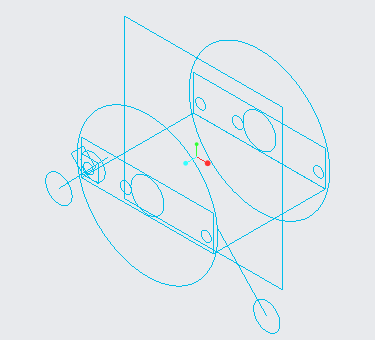
\includegraphics[width= .8\linewidth]{Design_Overview/Stabilization_Skeleton.PNG}
% \end{minipage}%
% \hfill
% \begin{minipage}{.48\textwidth}
%   \centering
%   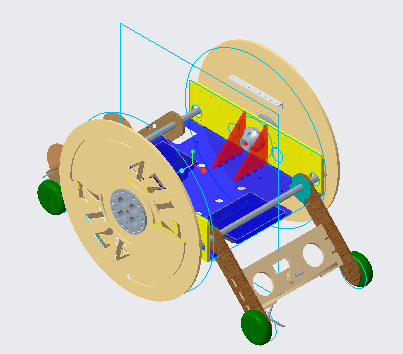
\includegraphics[width= .8\linewidth]{Design_Overview/Skel.PNG}
% \end{minipage}
% \end{figure}


\subsection*{Iterations}
Previously, the robot’s sides were made out of corrugated plastic and were purely cosmetic, serving no other purpose than to display our team numbers. To support our arms, we had a heavy assembly of REV extrusions which were both heavier and less stable than our current carbon fiber design. We chose carbon fiber for its superior strength to weight ratio, inspired by its use in aeronautical engineering on planes, marine engineering on boats, and even from its use of F1 racecars!
% Design_Sides_Image3

% \interesting{Design Iteration of the Stabilization Arms, Mark I to Mark V}{Design:4}

% \begin{figure}[h!]
% \centering
% 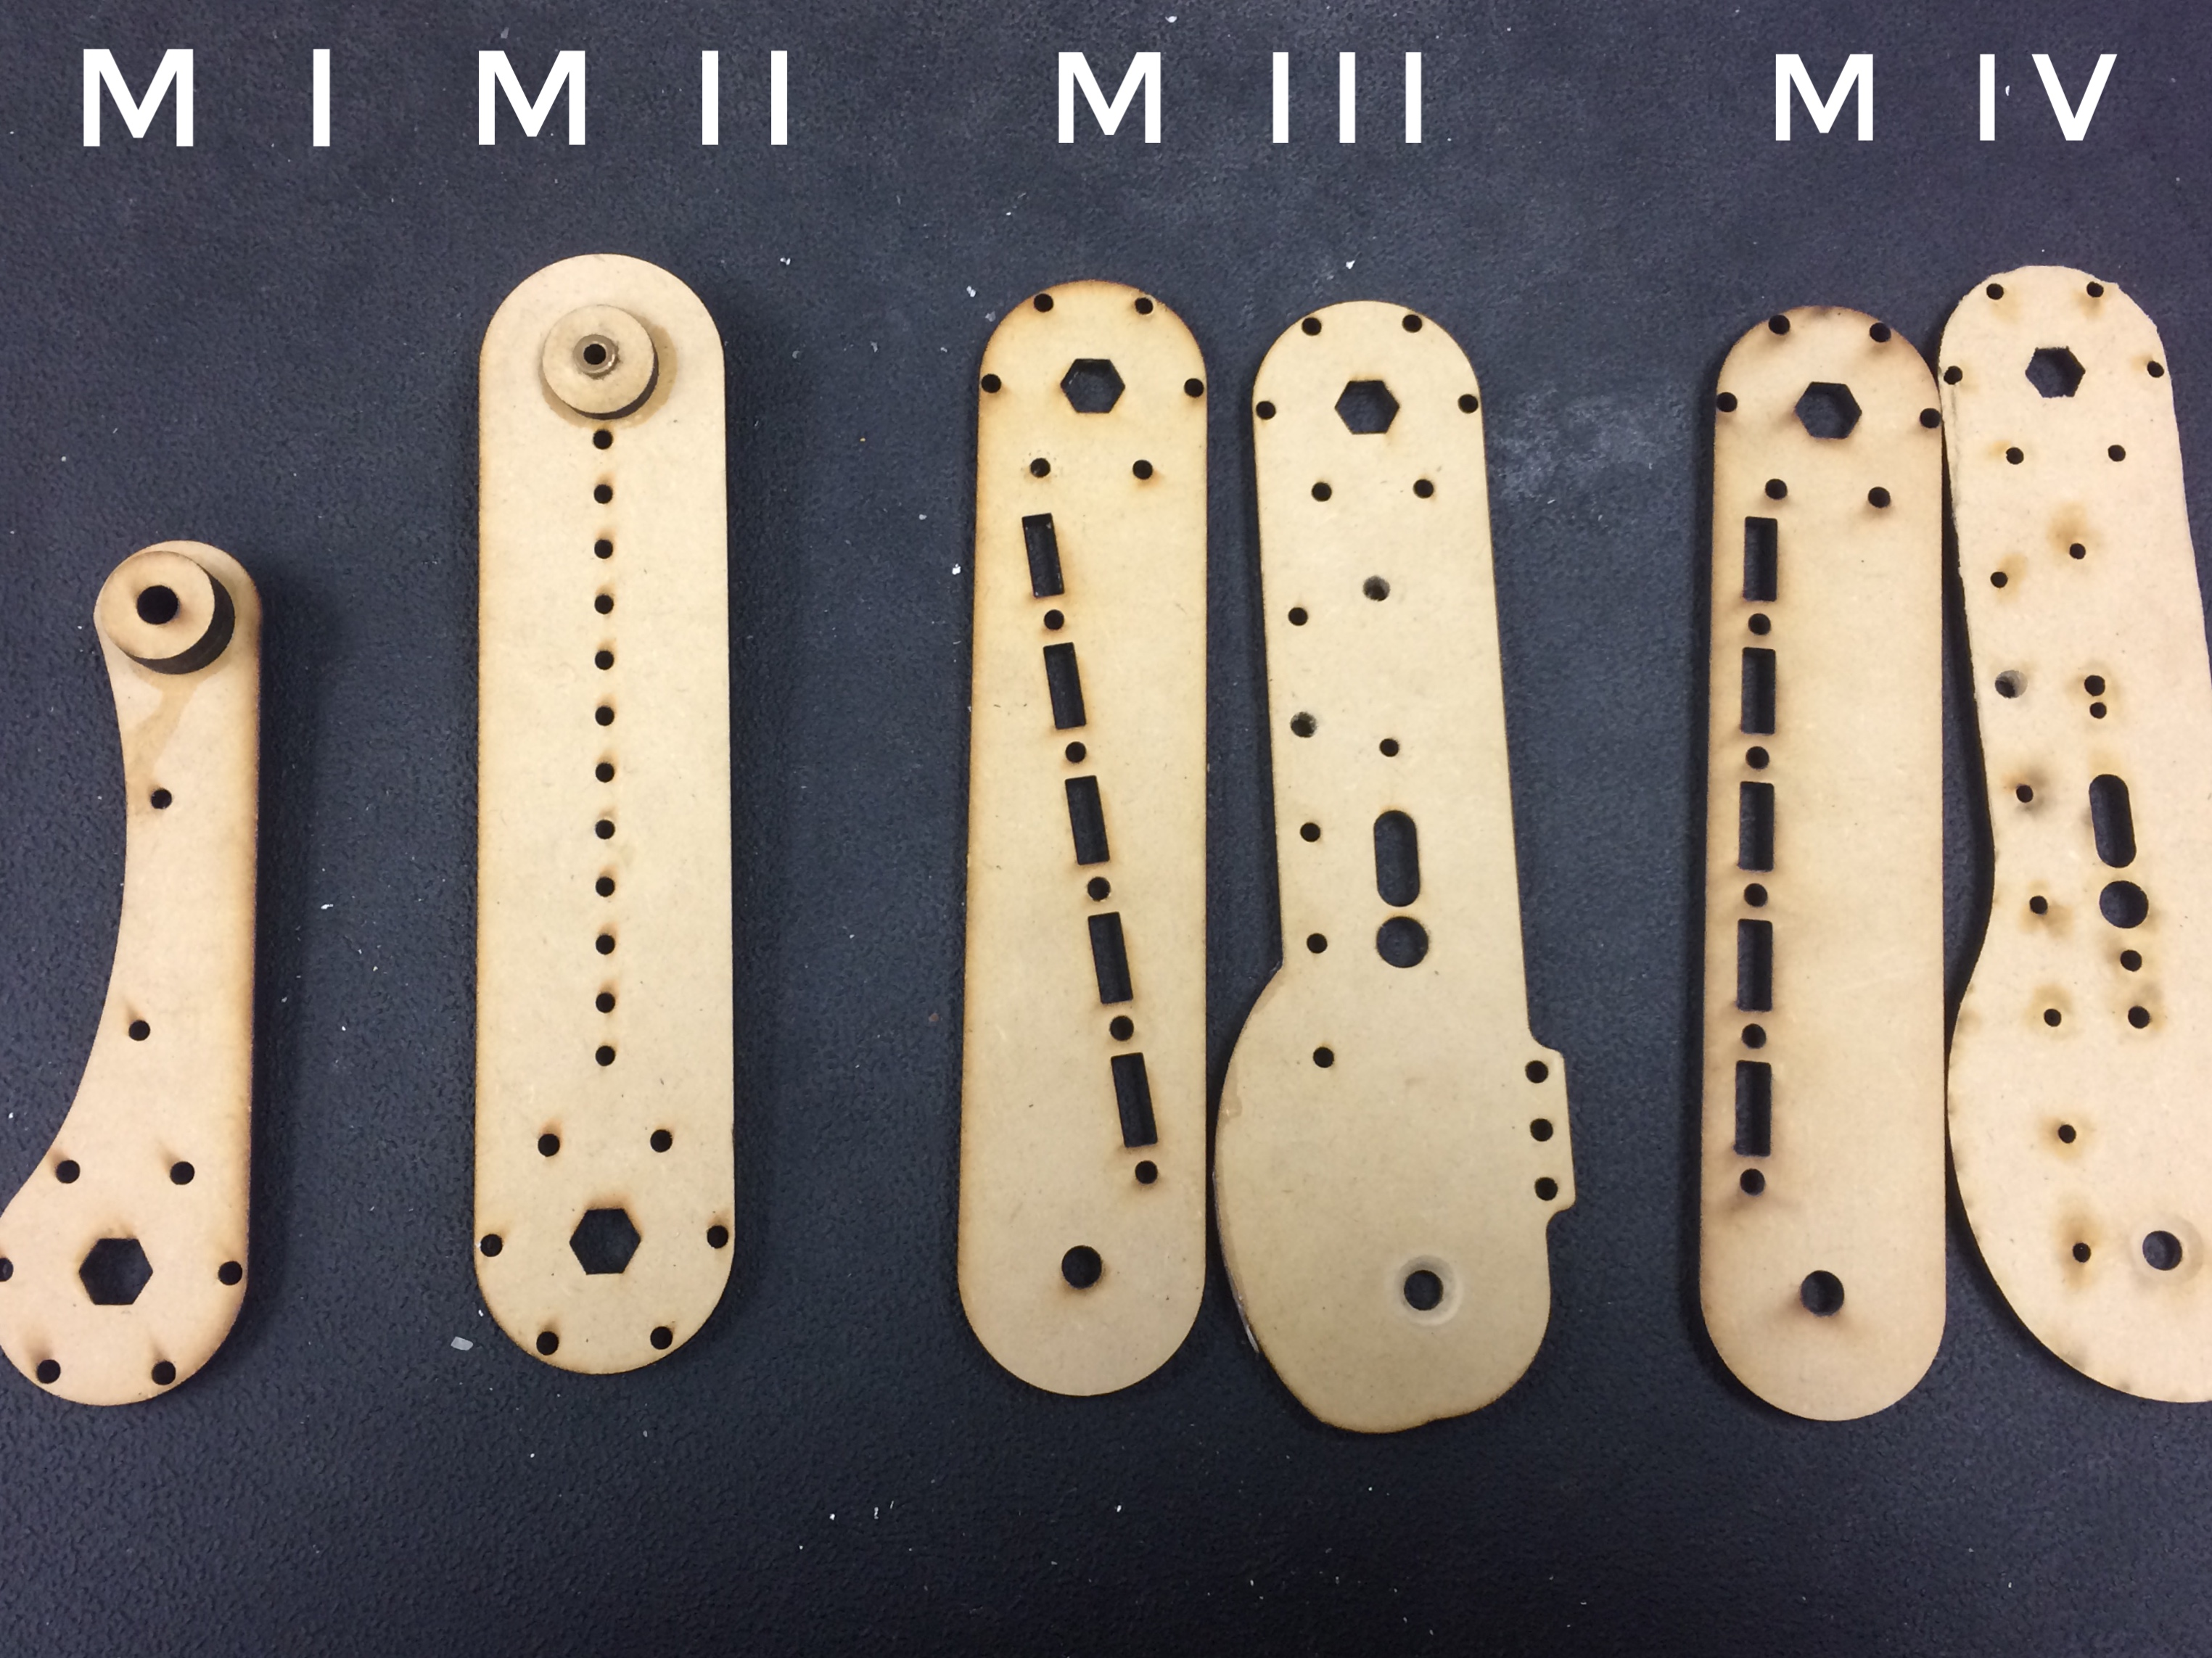
\includegraphics[width=.8\linewidth]{Design_Overview/Iteration.jpg}
% \caption{Design Iteration of the Stabilization Arms, Mark I to IV}
% \label{fig:iteration}
% \end{figure}

% \begin{figure}[h!]
% \centering
% \begin{minipage}{.32\textwidth}
%   \centering
%   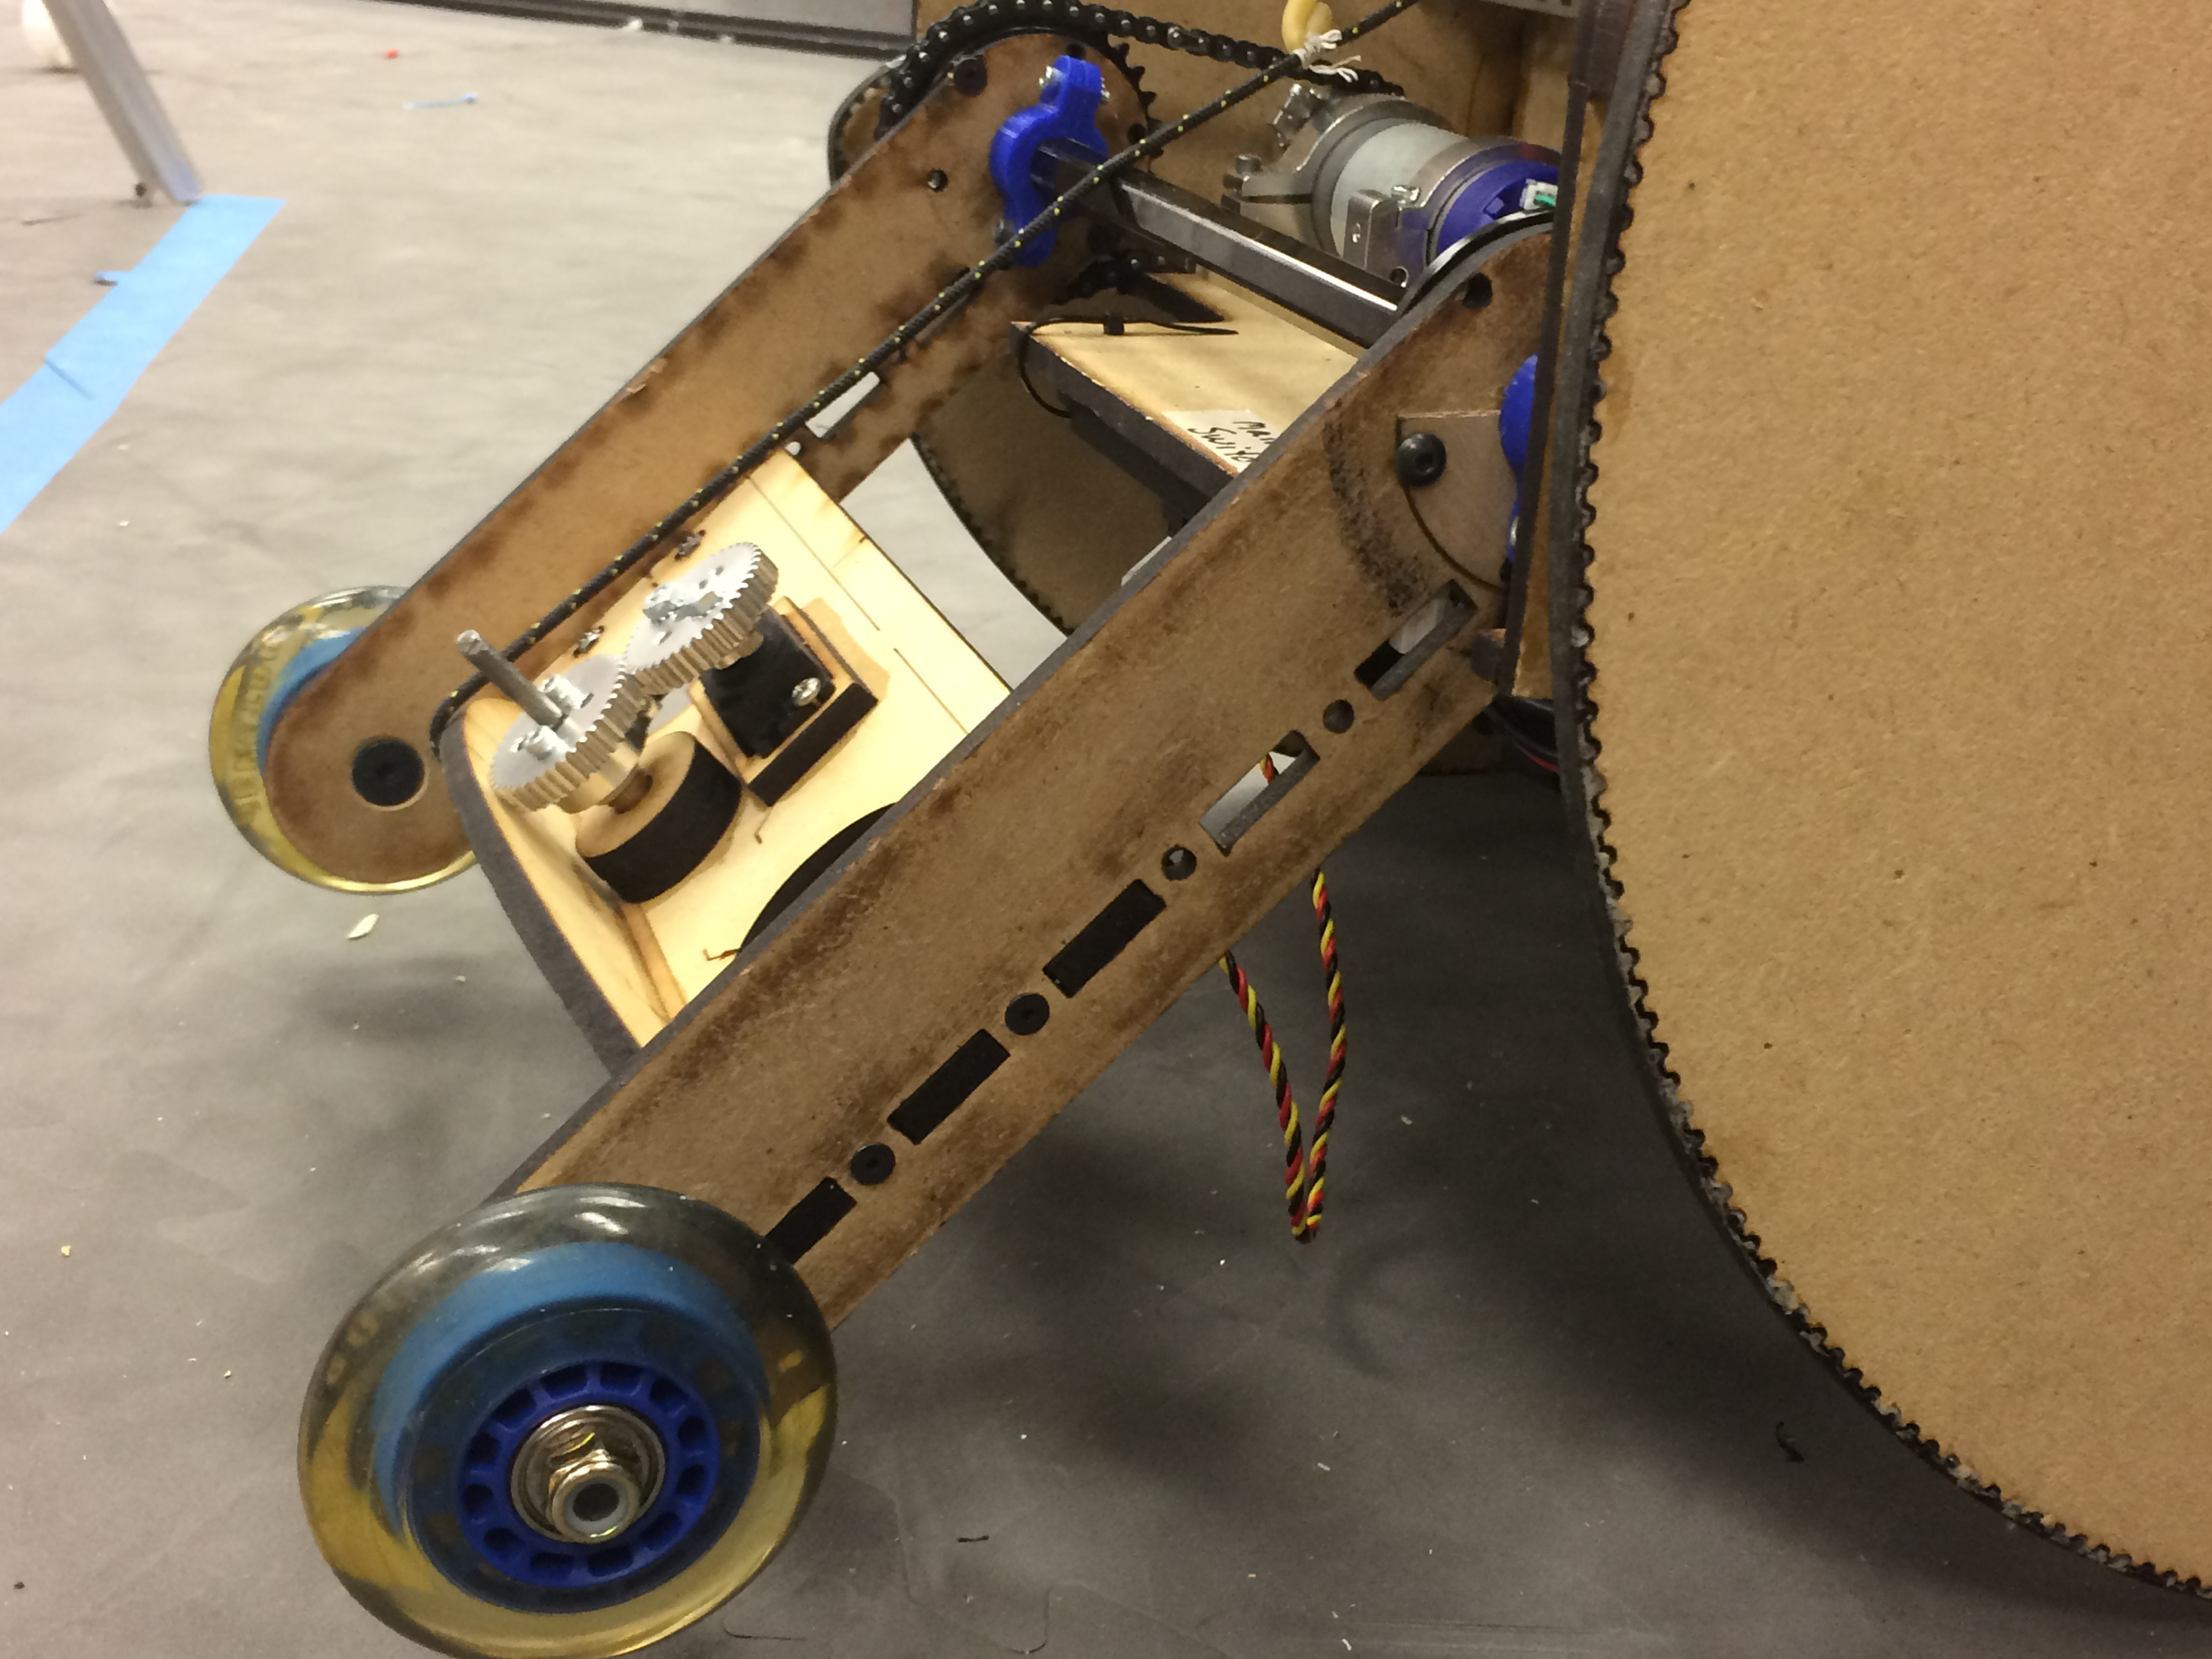
\includegraphics[width= .9\linewidth]{Design_Overview/front_arm.JPG}
% \end{minipage}%
% \hfill
% \begin{minipage}{.32\textwidth}
%   \centering
%   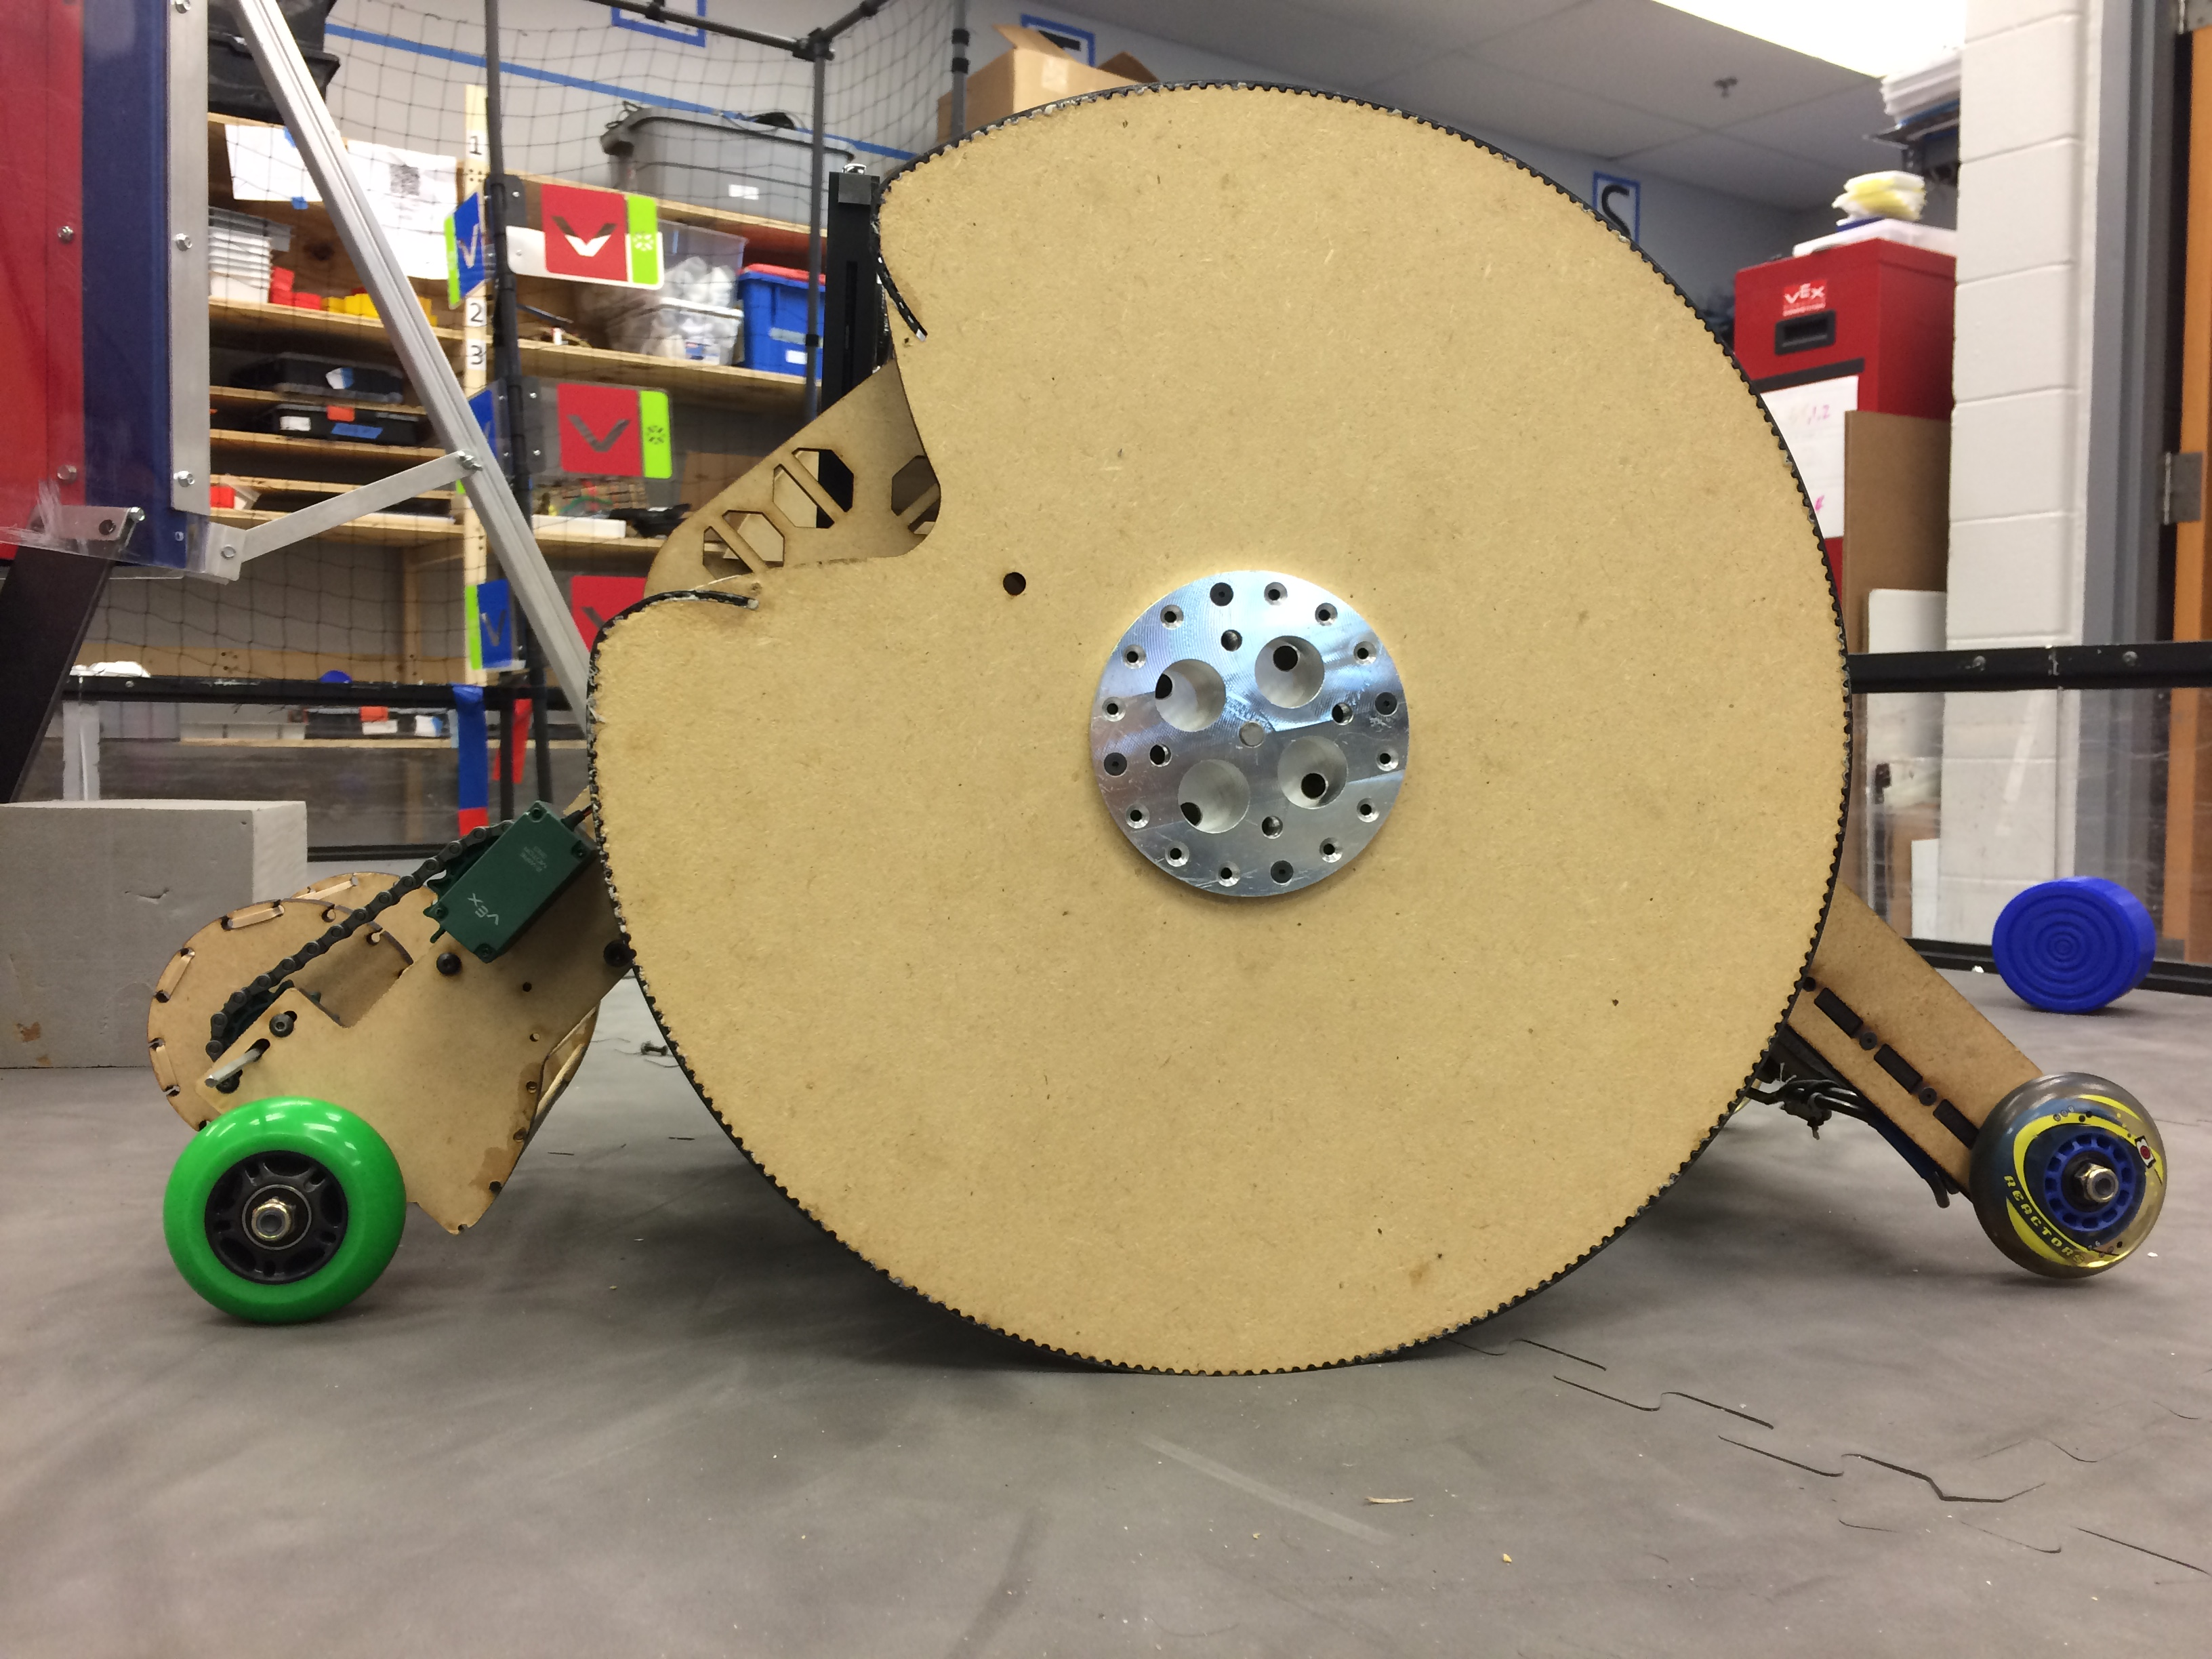
\includegraphics[width= .9\linewidth]{Design_Overview/both_arms.JPG}
% 	\caption{Final Stabilization Arms, Mark V}
% 	\label{fig:Triple_Arm_IMG}
% \end{minipage}%
% 	\hfill
% \begin{minipage}{.32\textwidth}
%   \centering
%   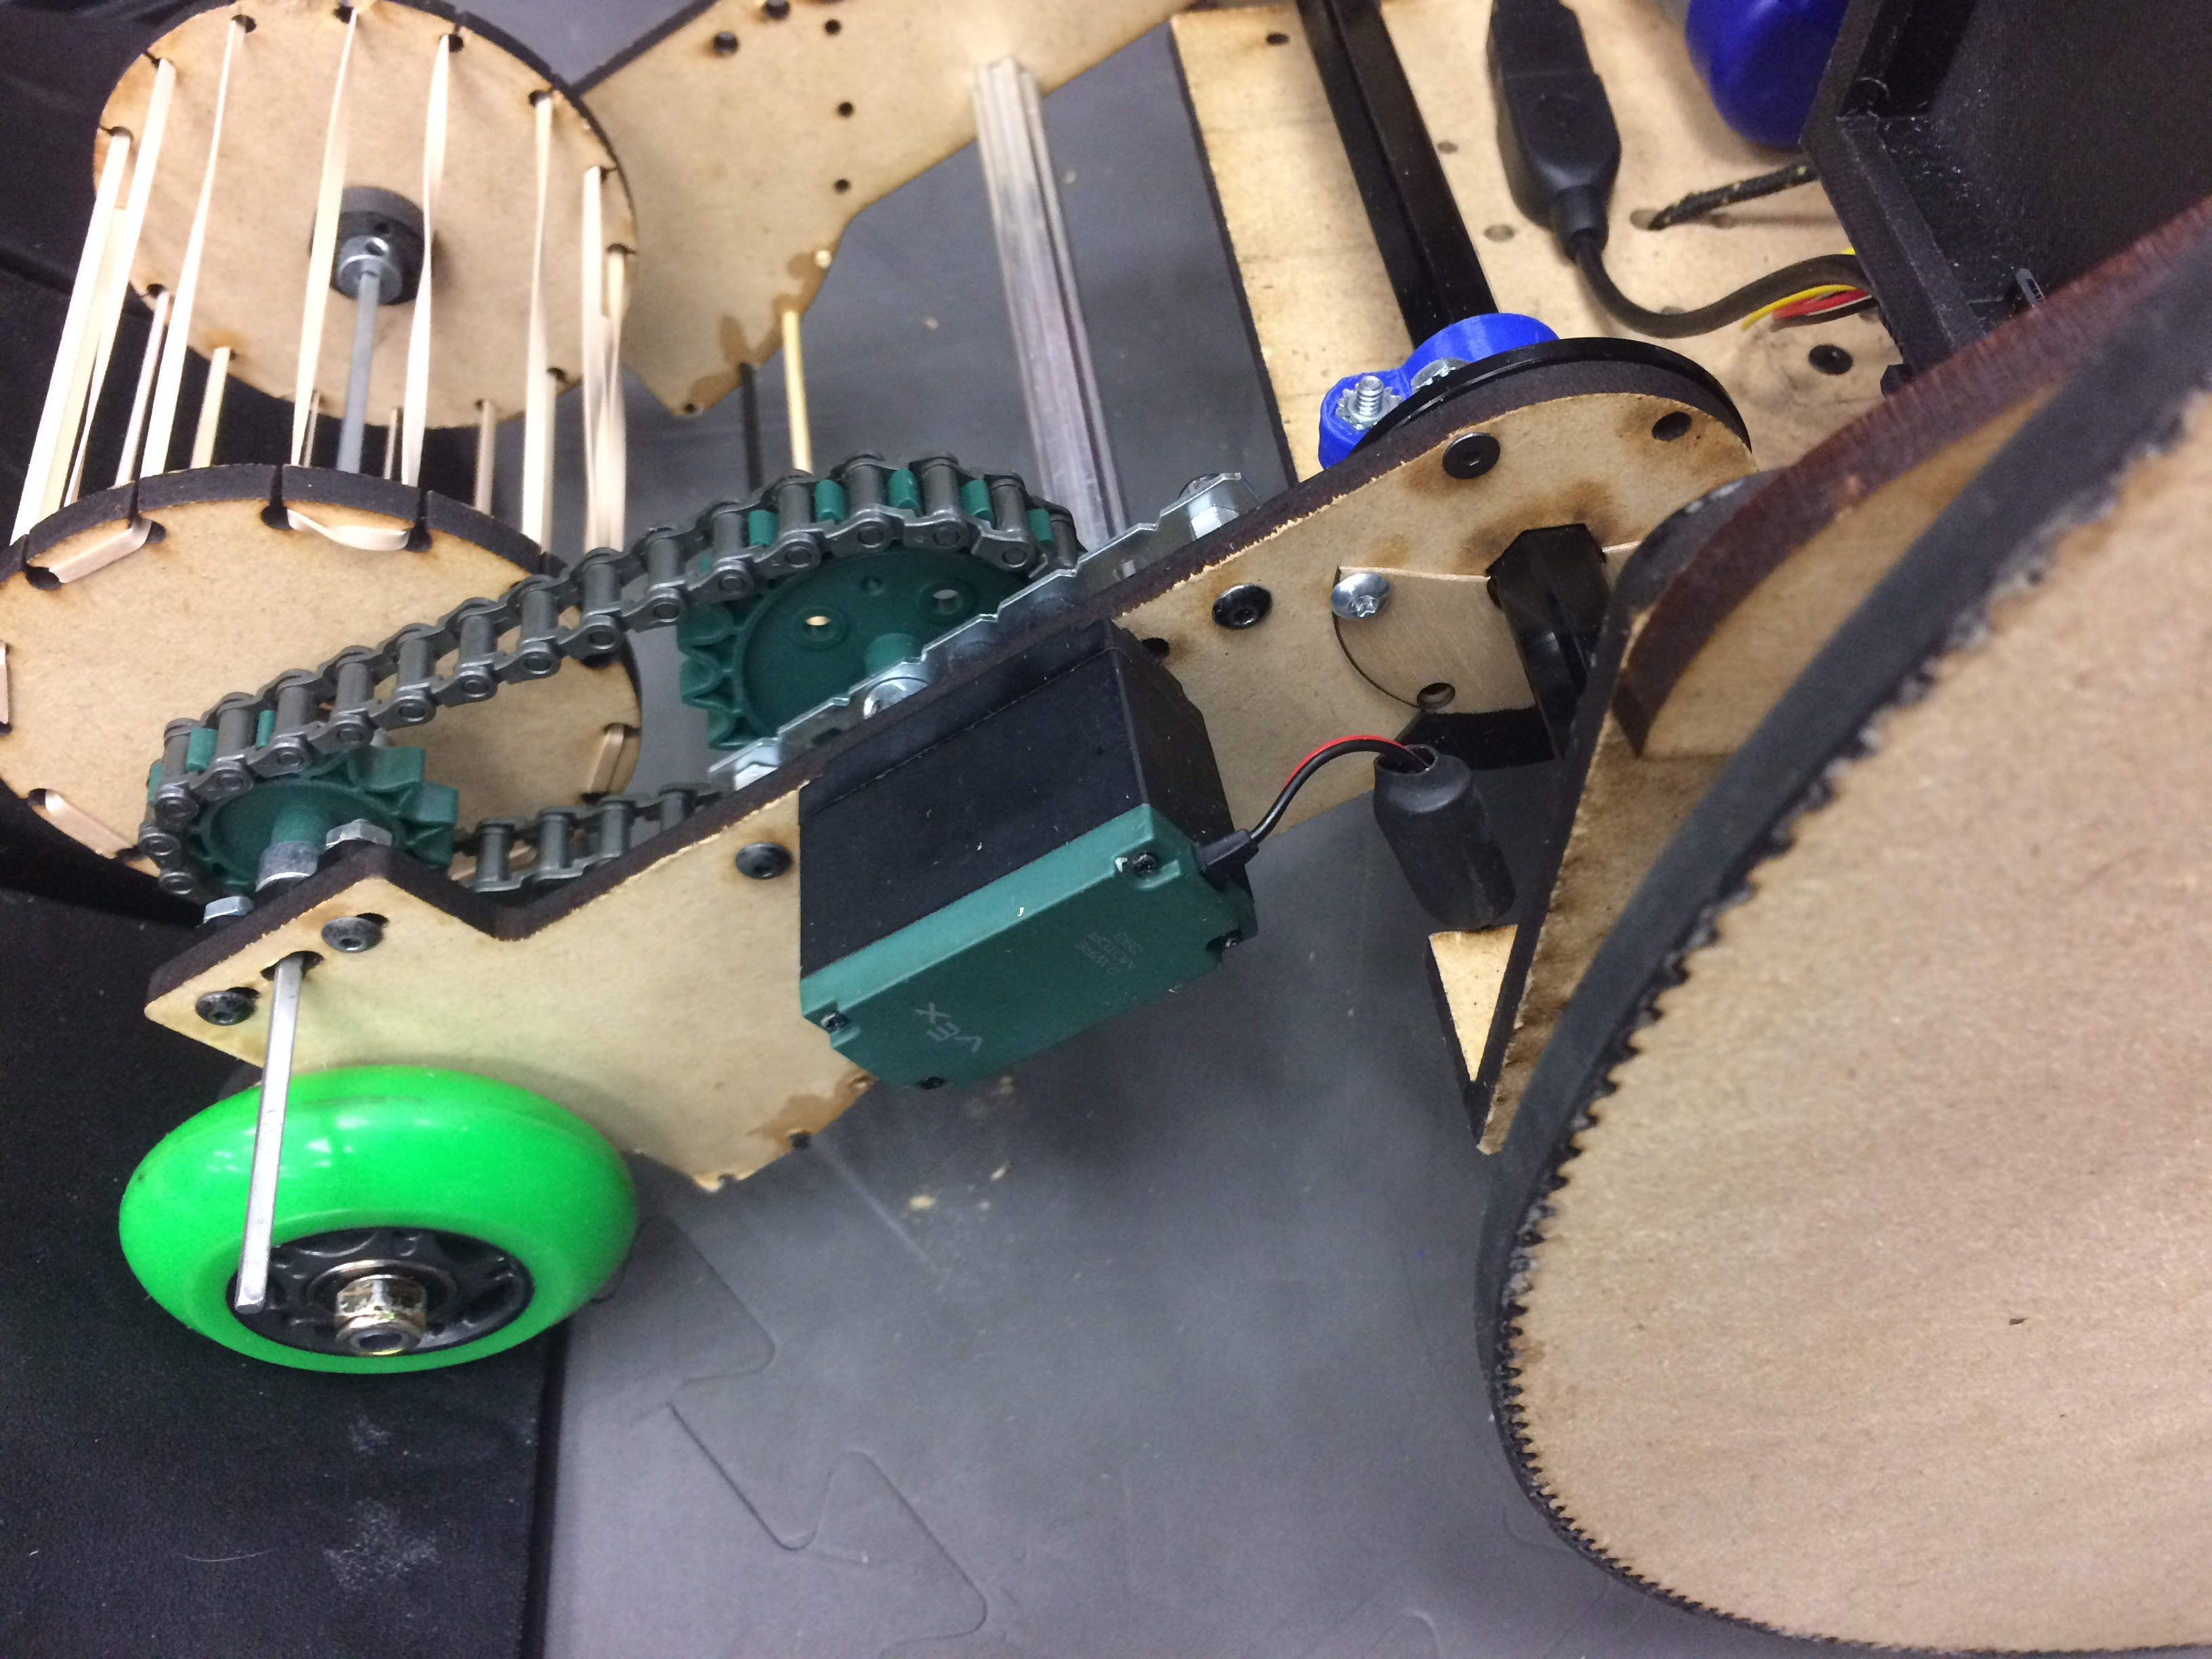
\includegraphics[width= .9\linewidth]{Design_Overview/rear_arm.JPG}
% \end{minipage}
% \end{figure}

\subsection*{Sensors and Control}
As you may imagine, an arm swinging all around may cause your robot to tip over and we had many issues with this at the beginning of the season. To combat this, we decided to use the sine function in concordance with a PID algorithm to reach a targeted destination. The error sent to the PID controller comes from the REV Hex Motor’s built in encoder. The PID algorithm would be getting the arm to the position, and the sine function would be slowing the arm down as it reached the top, which is where it would have the most momentum. This allowed us to be fast with our arm, but slow down in time. Several diagrams explaining this are shown below.

% Image: Design_Arm_ArmPidGraph
% Design_Arm_FBD


%\begin{figure}[h!]
%\centering
%\begin{minipage}{.48\textwidth}
%  \centering
%  \includegraphics[width= .8\linewidth, angle=-90]{Meetings/January/01-21-19/interrupter.png}
%\end{minipage}%
%\hfill
%\begin{minipage}{.48\textwidth}
 % \centering
%  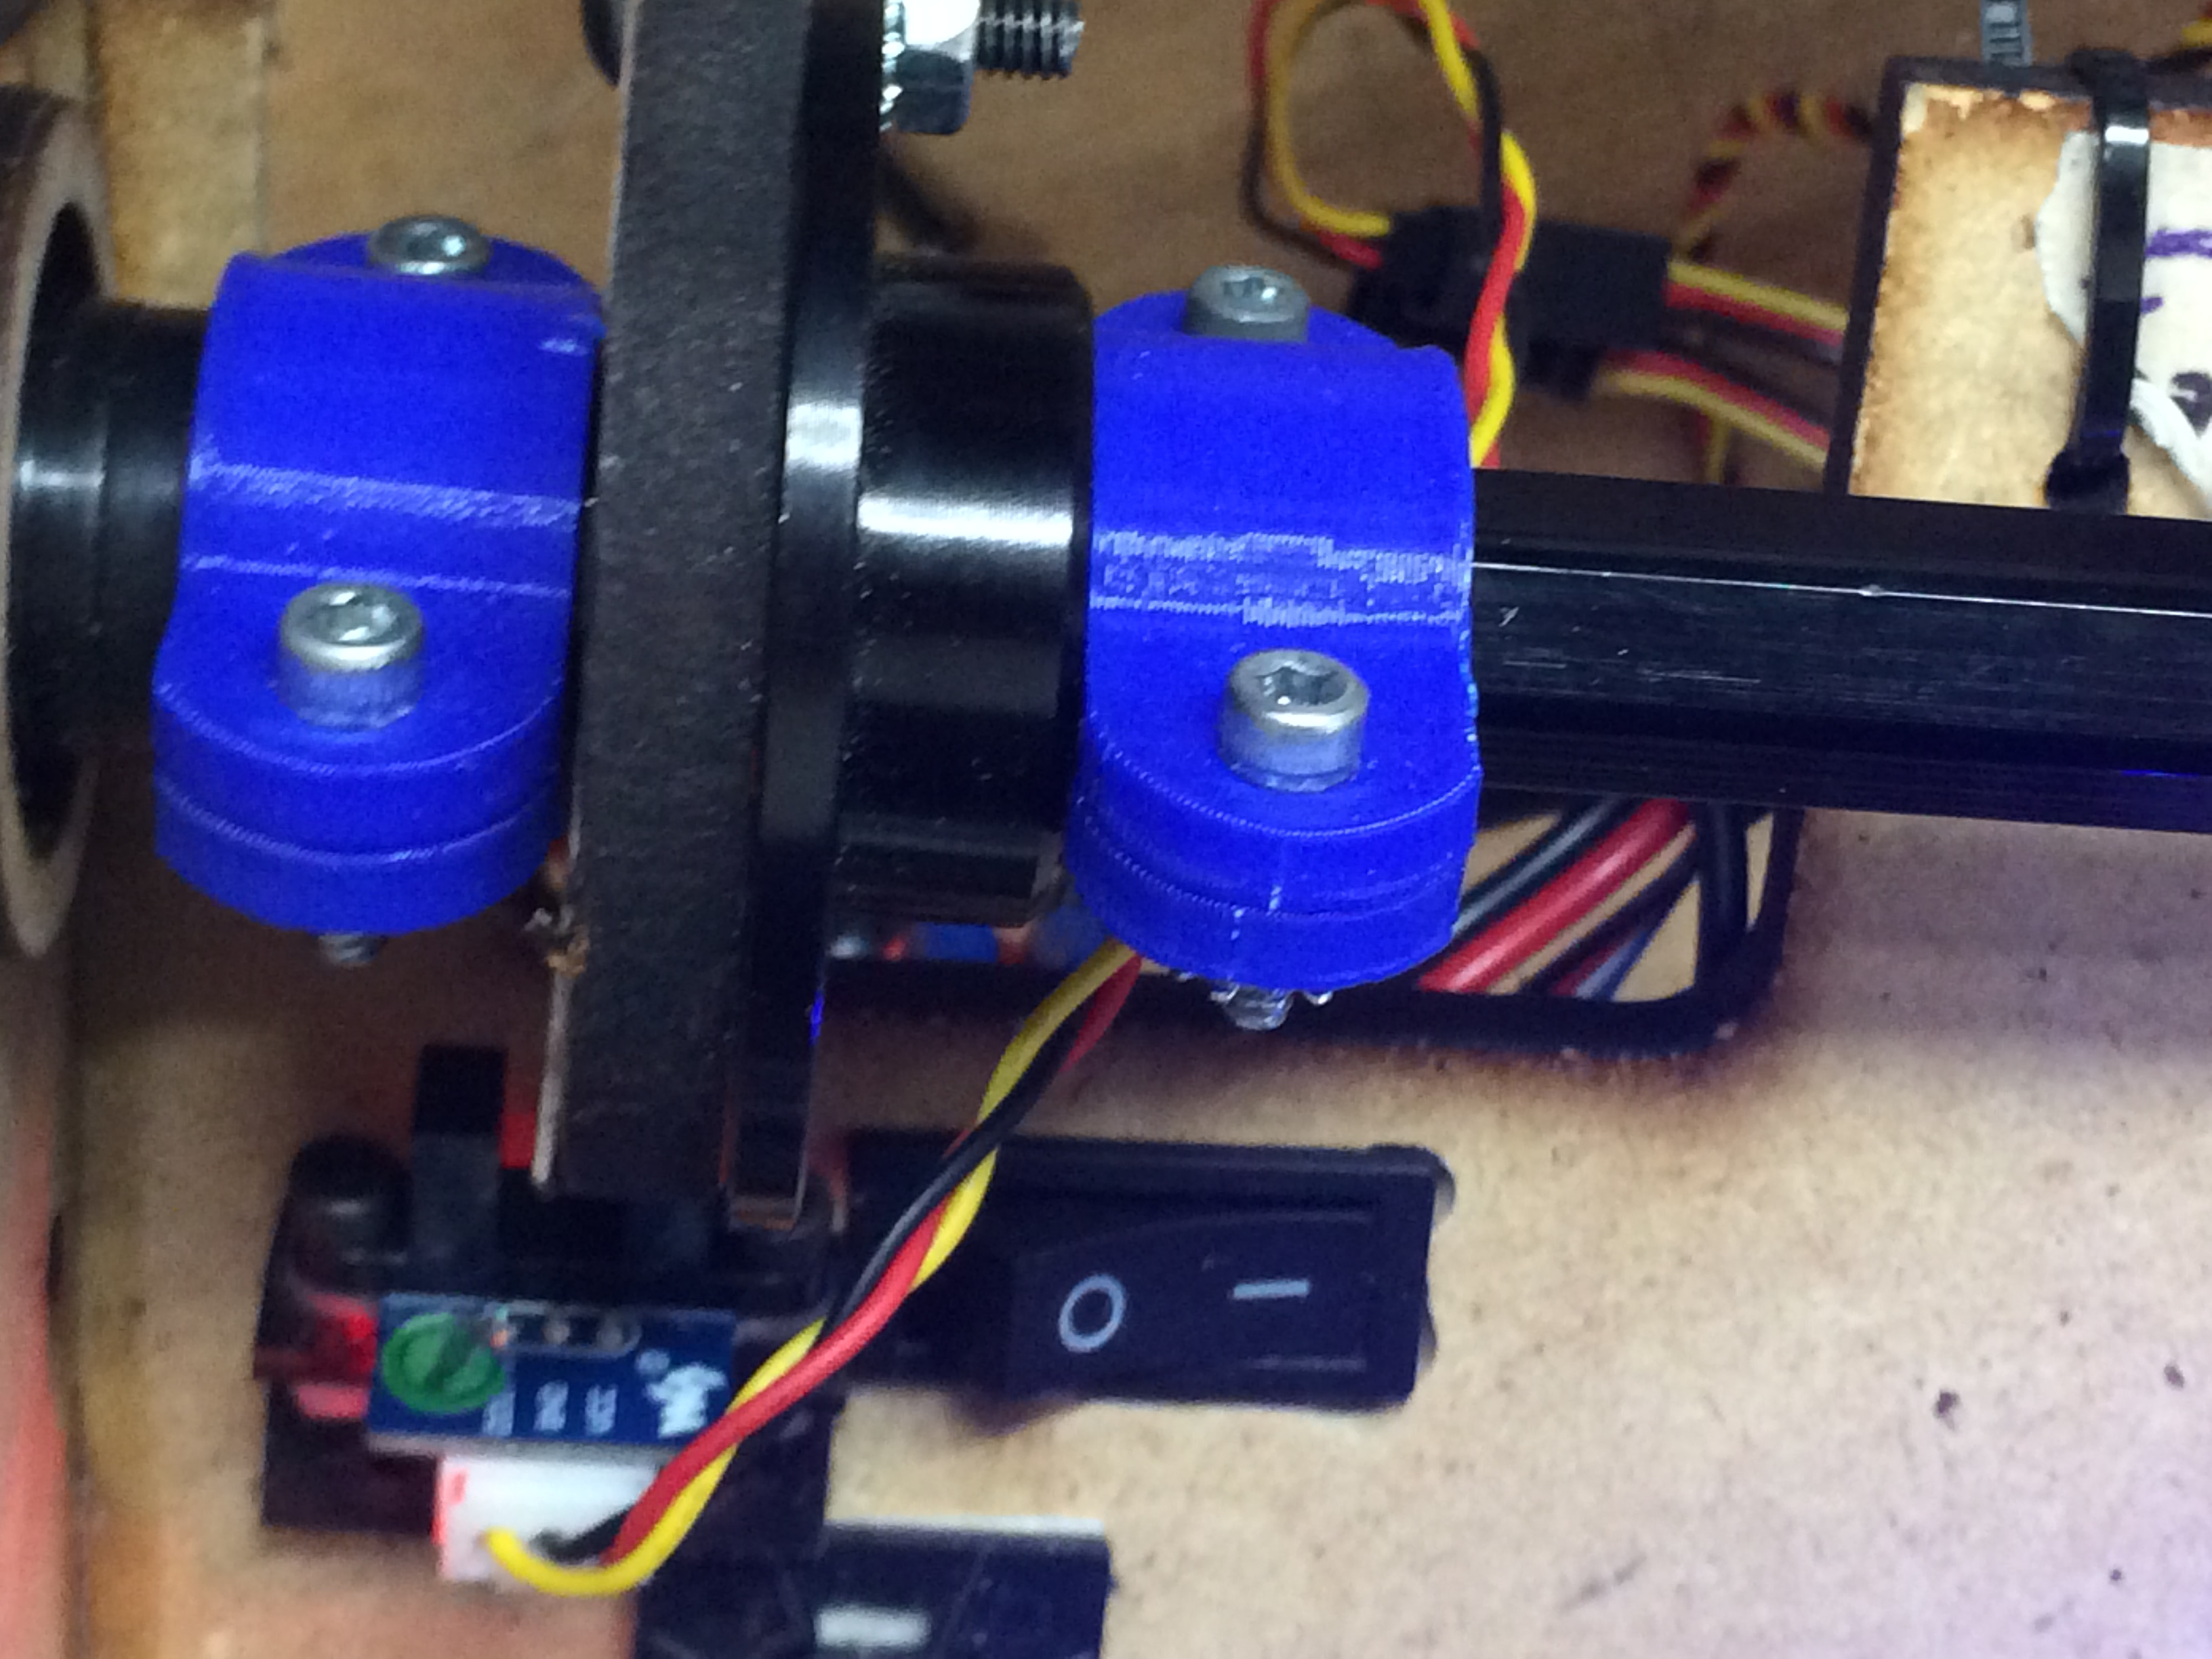
\includegraphics[width= .75\linewidth, angle=-90]{Design_Overview/photo_int_real.JPG}
%\end{minipage}
%\end{figure}

% \vskip 0.35in
% \textbf{Different Arm Preset Positions:}
% \textit{Various Preset Positions for the Stabilizing Arms}

% \interesting{Various Preset Positions for the Arms}{control:3}

% \begin{figure}[h!]
% \centering
% \begin{minipage}{.32\textwidth}
%   \centering
%   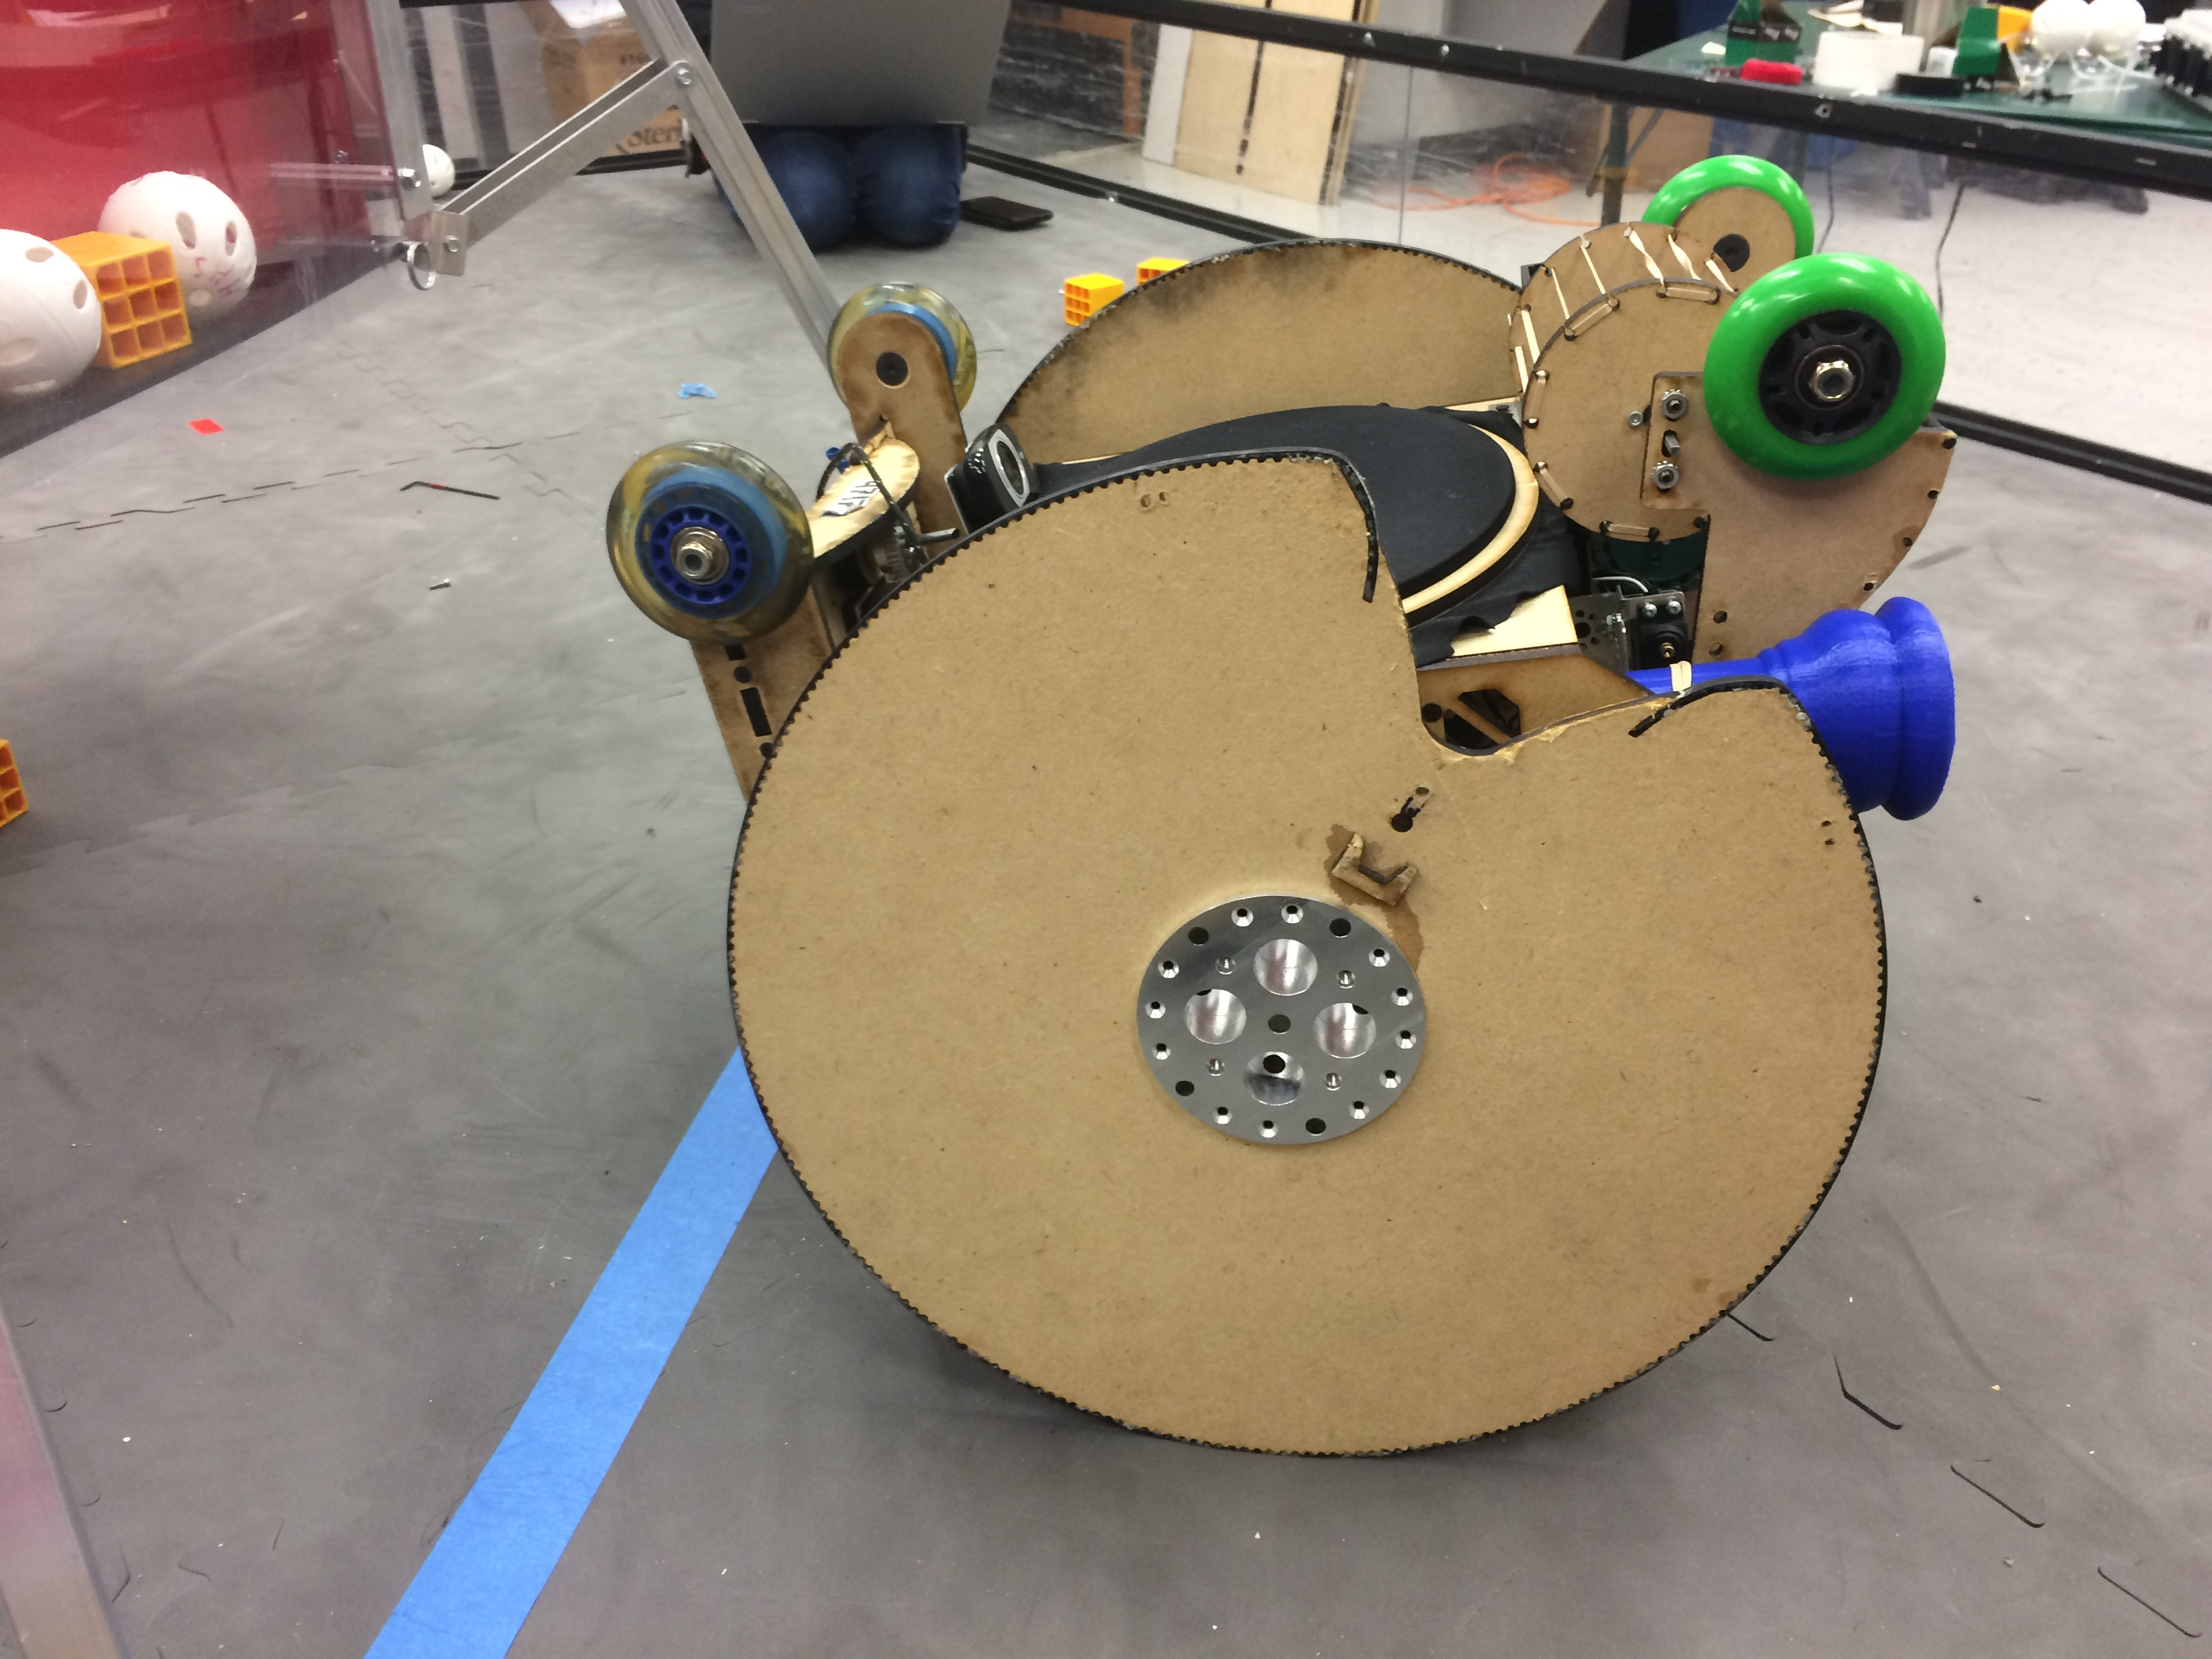
\includegraphics[width= .9\linewidth]{Design_Overview/Zero.JPG} %%zero
% \end{minipage}%
% \hfill
% \begin{minipage}{.32\textwidth}
%   \centering
%   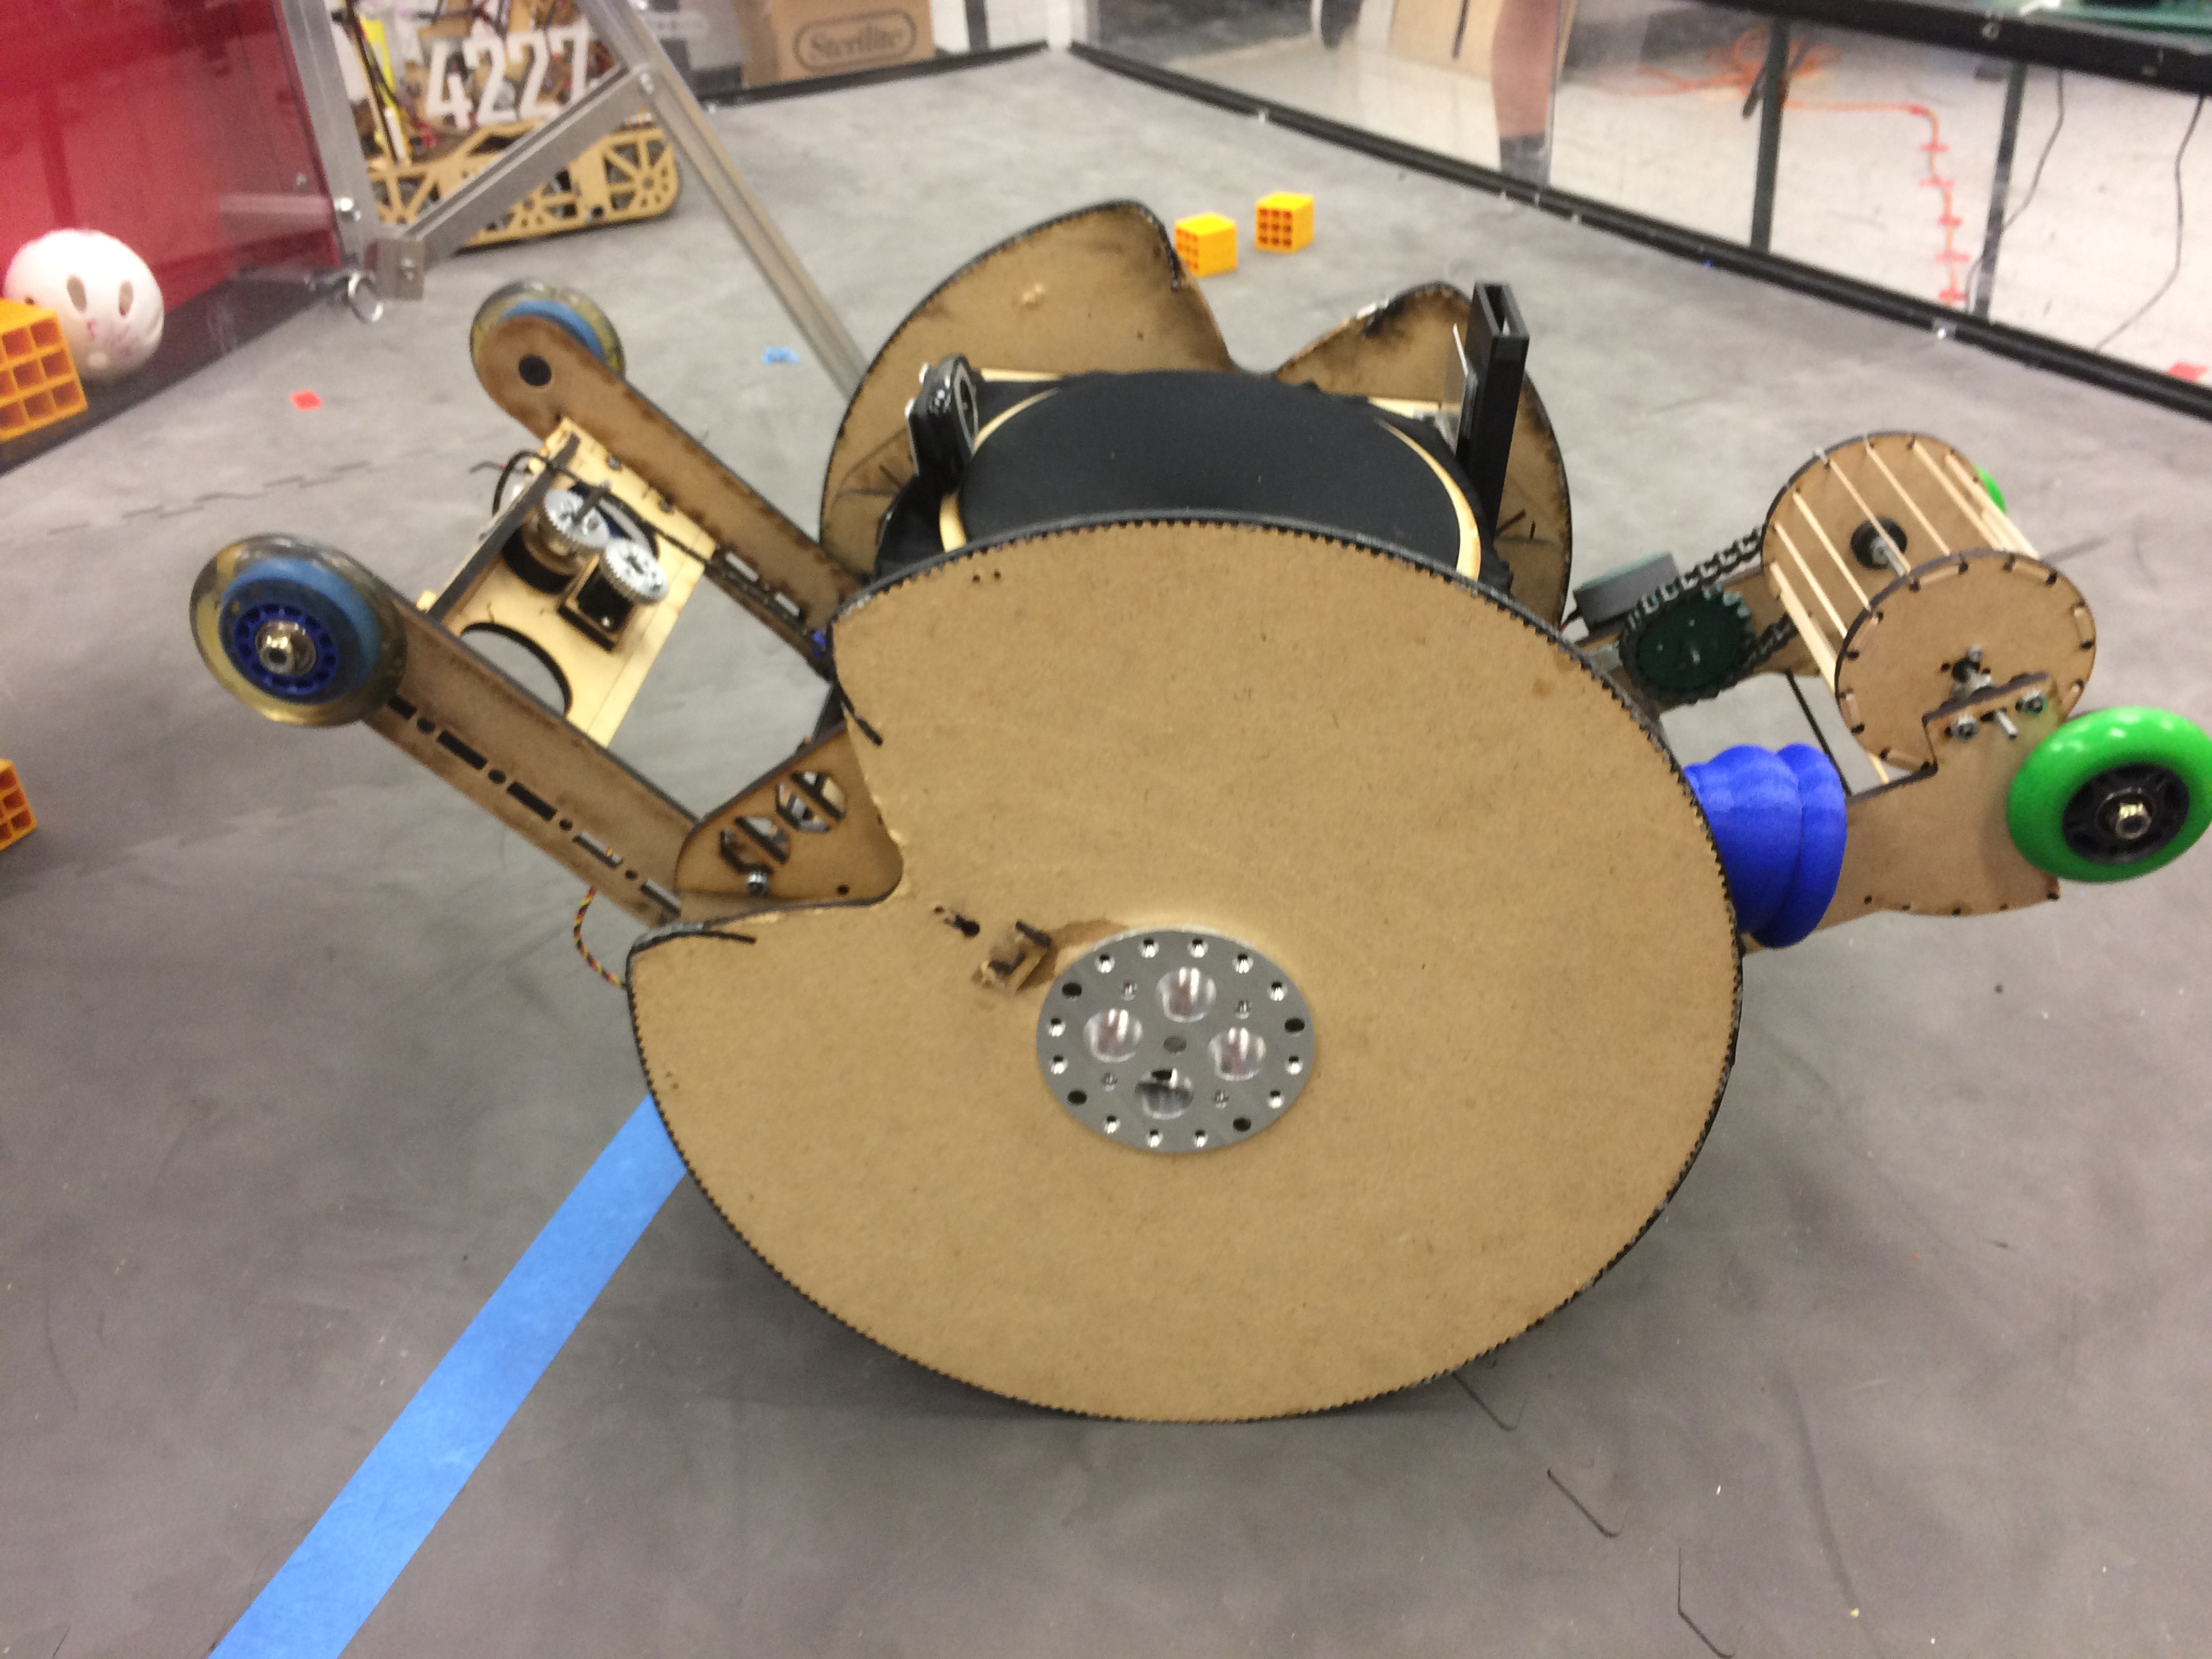
\includegraphics[width= .9\linewidth]{Design_Overview/45.JPG} %%45
% \end{minipage}%
%   \hfill
% \begin{minipage}{.32\textwidth}
%   \centering
%   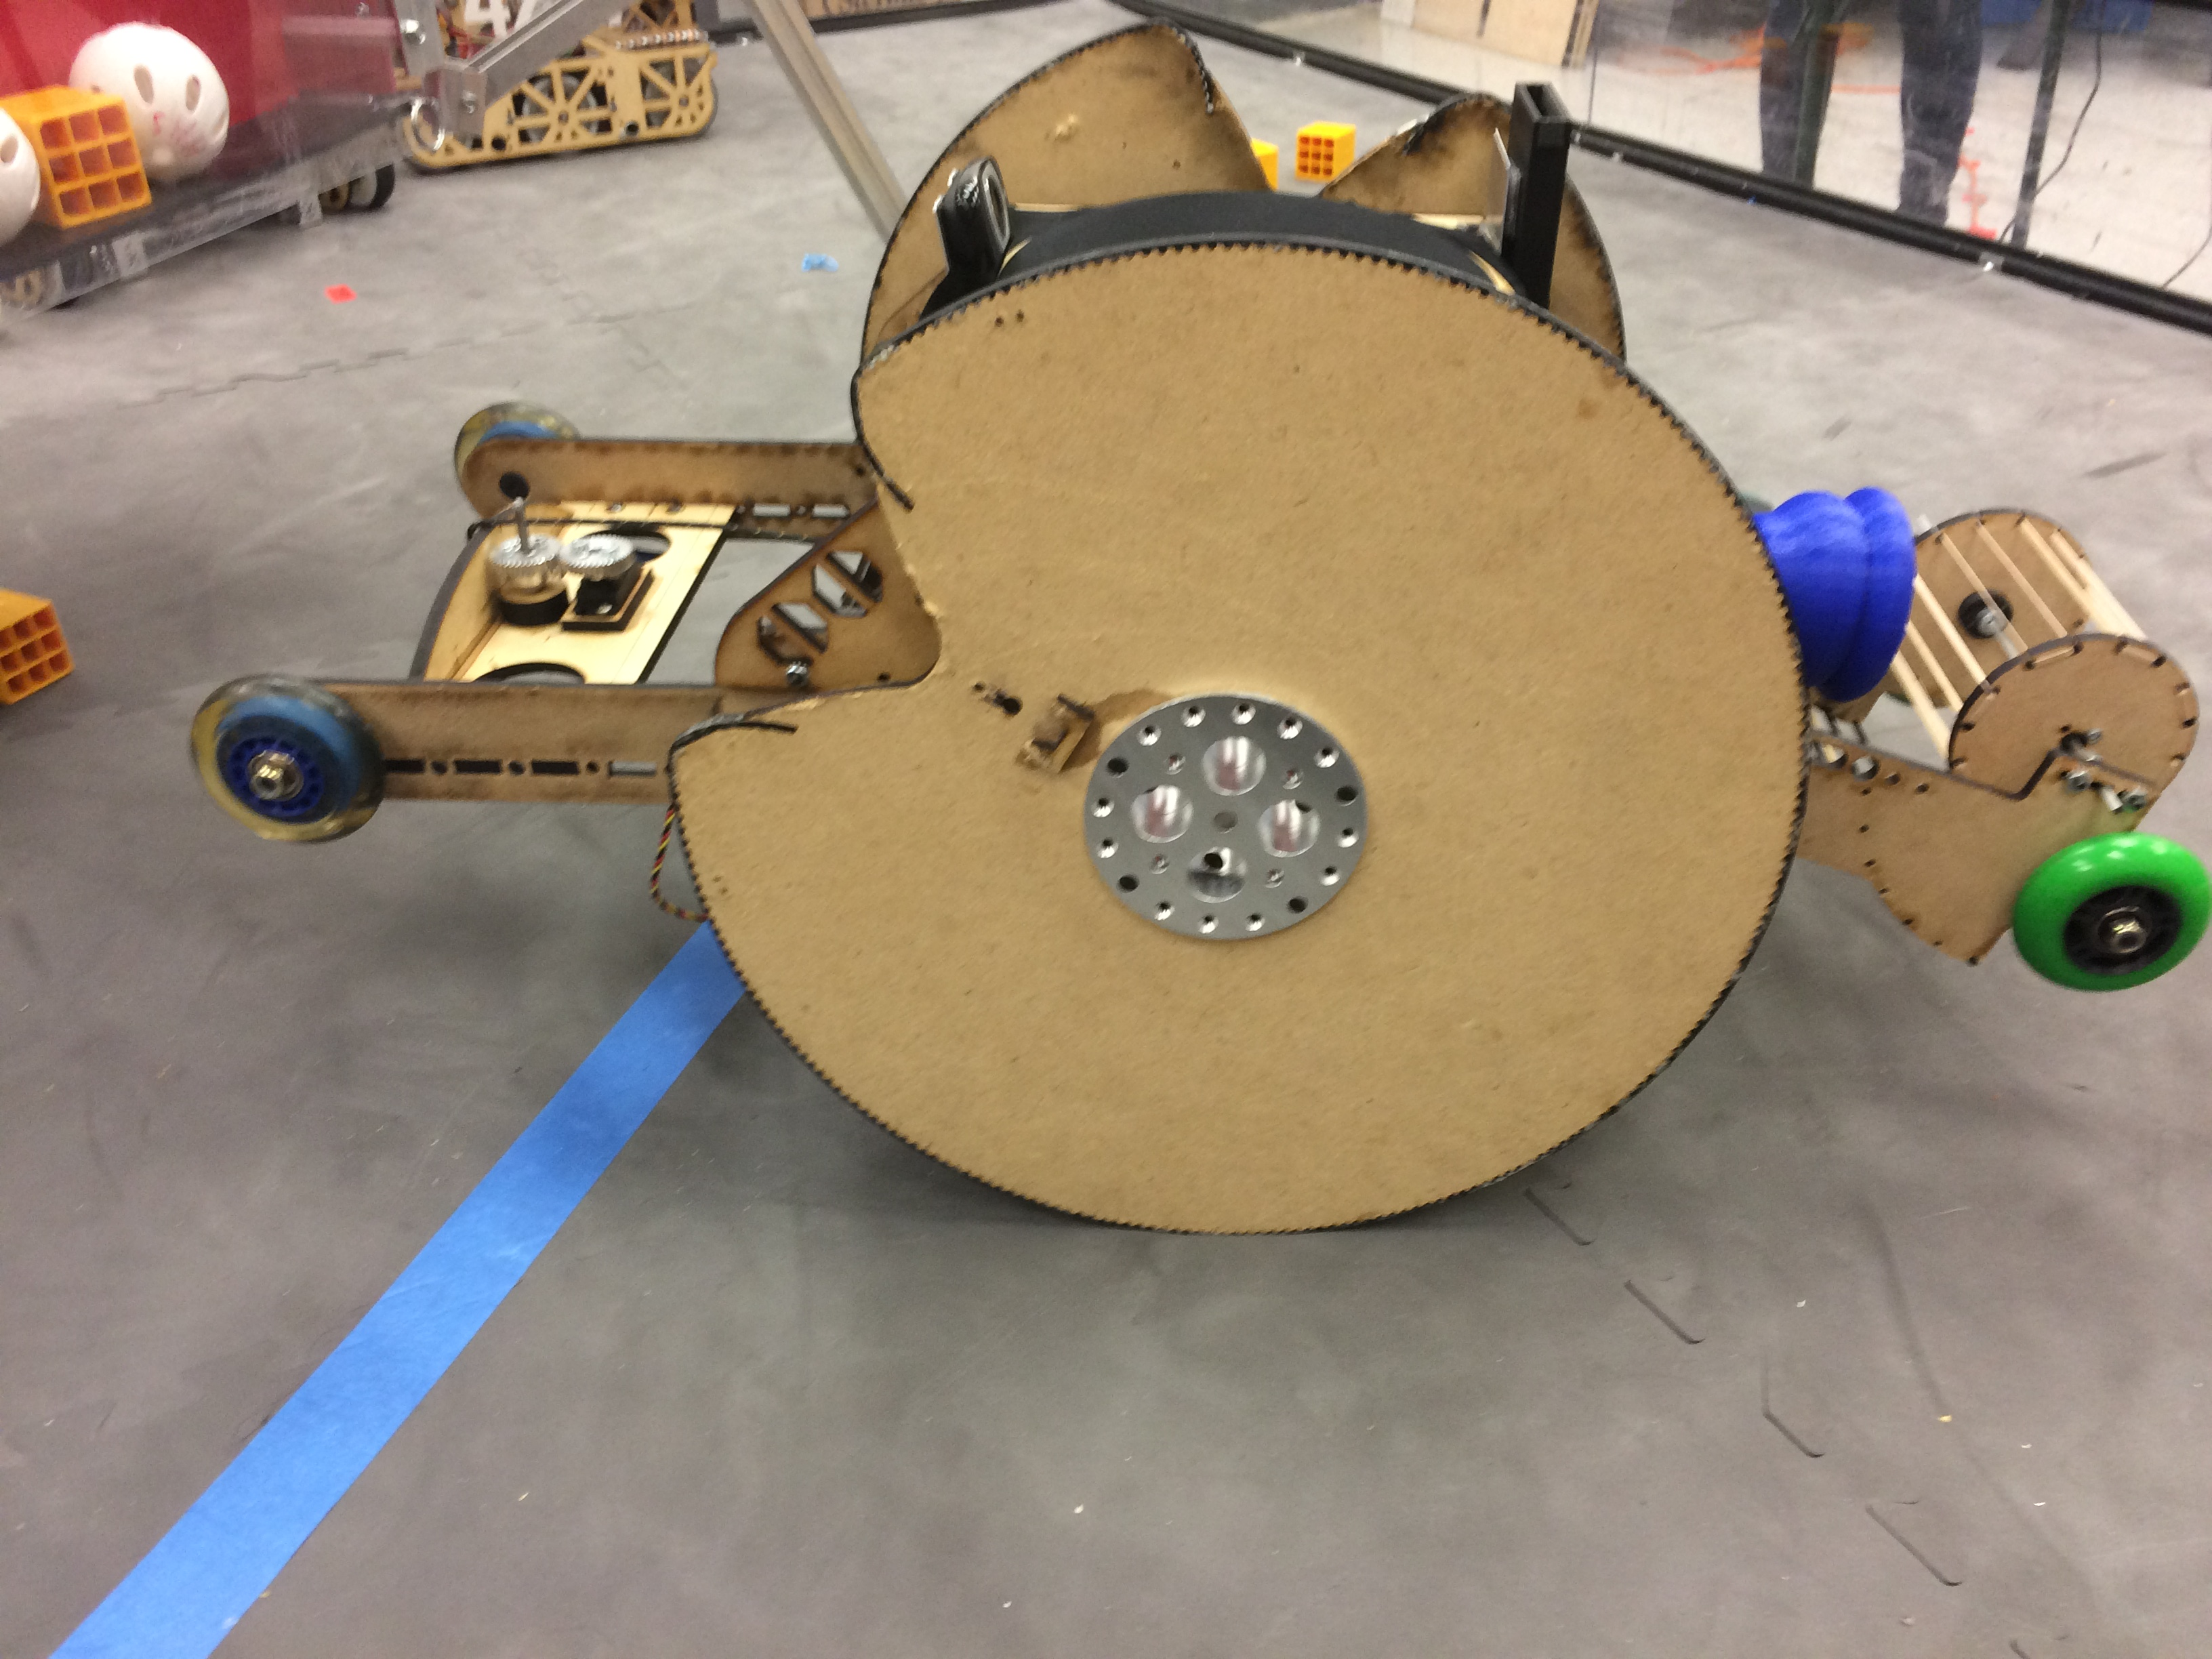
\includegraphics[width= .9\linewidth]{Design_Overview/90.JPG} %%90
% \end{minipage}
% \end{figure}

% \begin{figure}[h!]
% \centering
% \begin{minipage}{.32\textwidth}
%   \centering
%   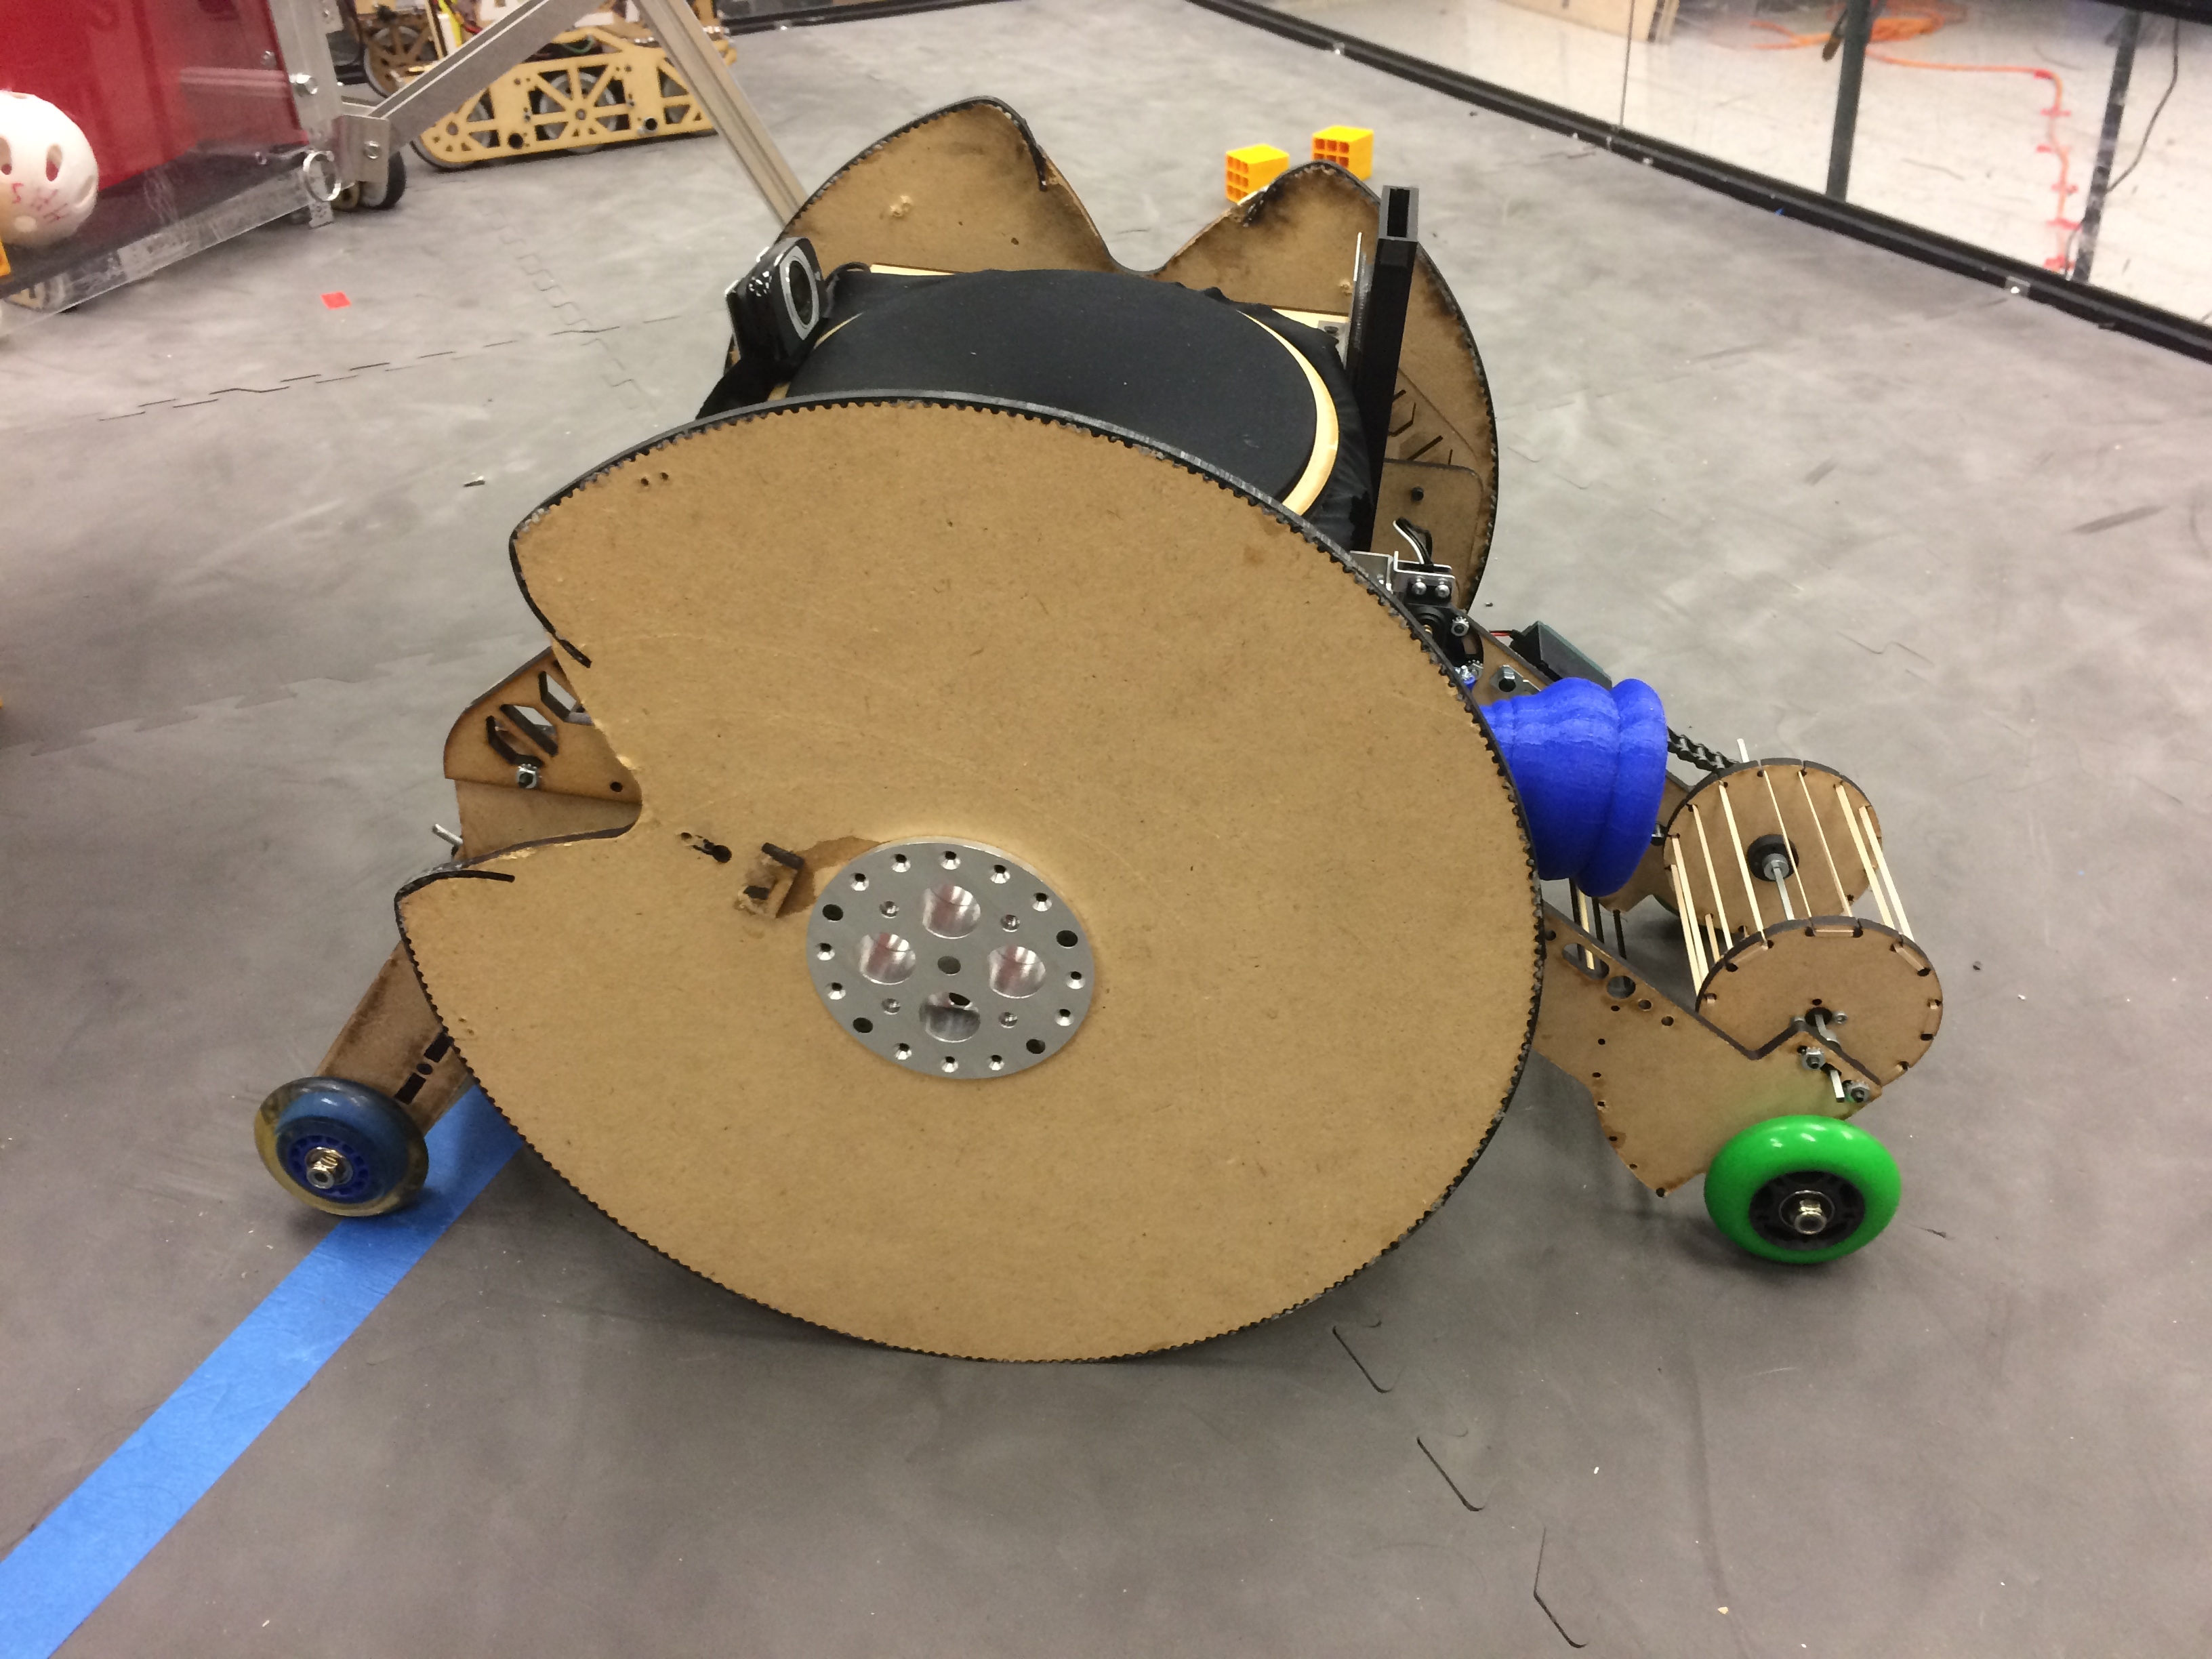
\includegraphics[width= .9\linewidth]{Design_Overview/Natural.JPG} %%natural
% \end{minipage}%
% \hfill
% \begin{minipage}{.32\textwidth}
%   \centering
%   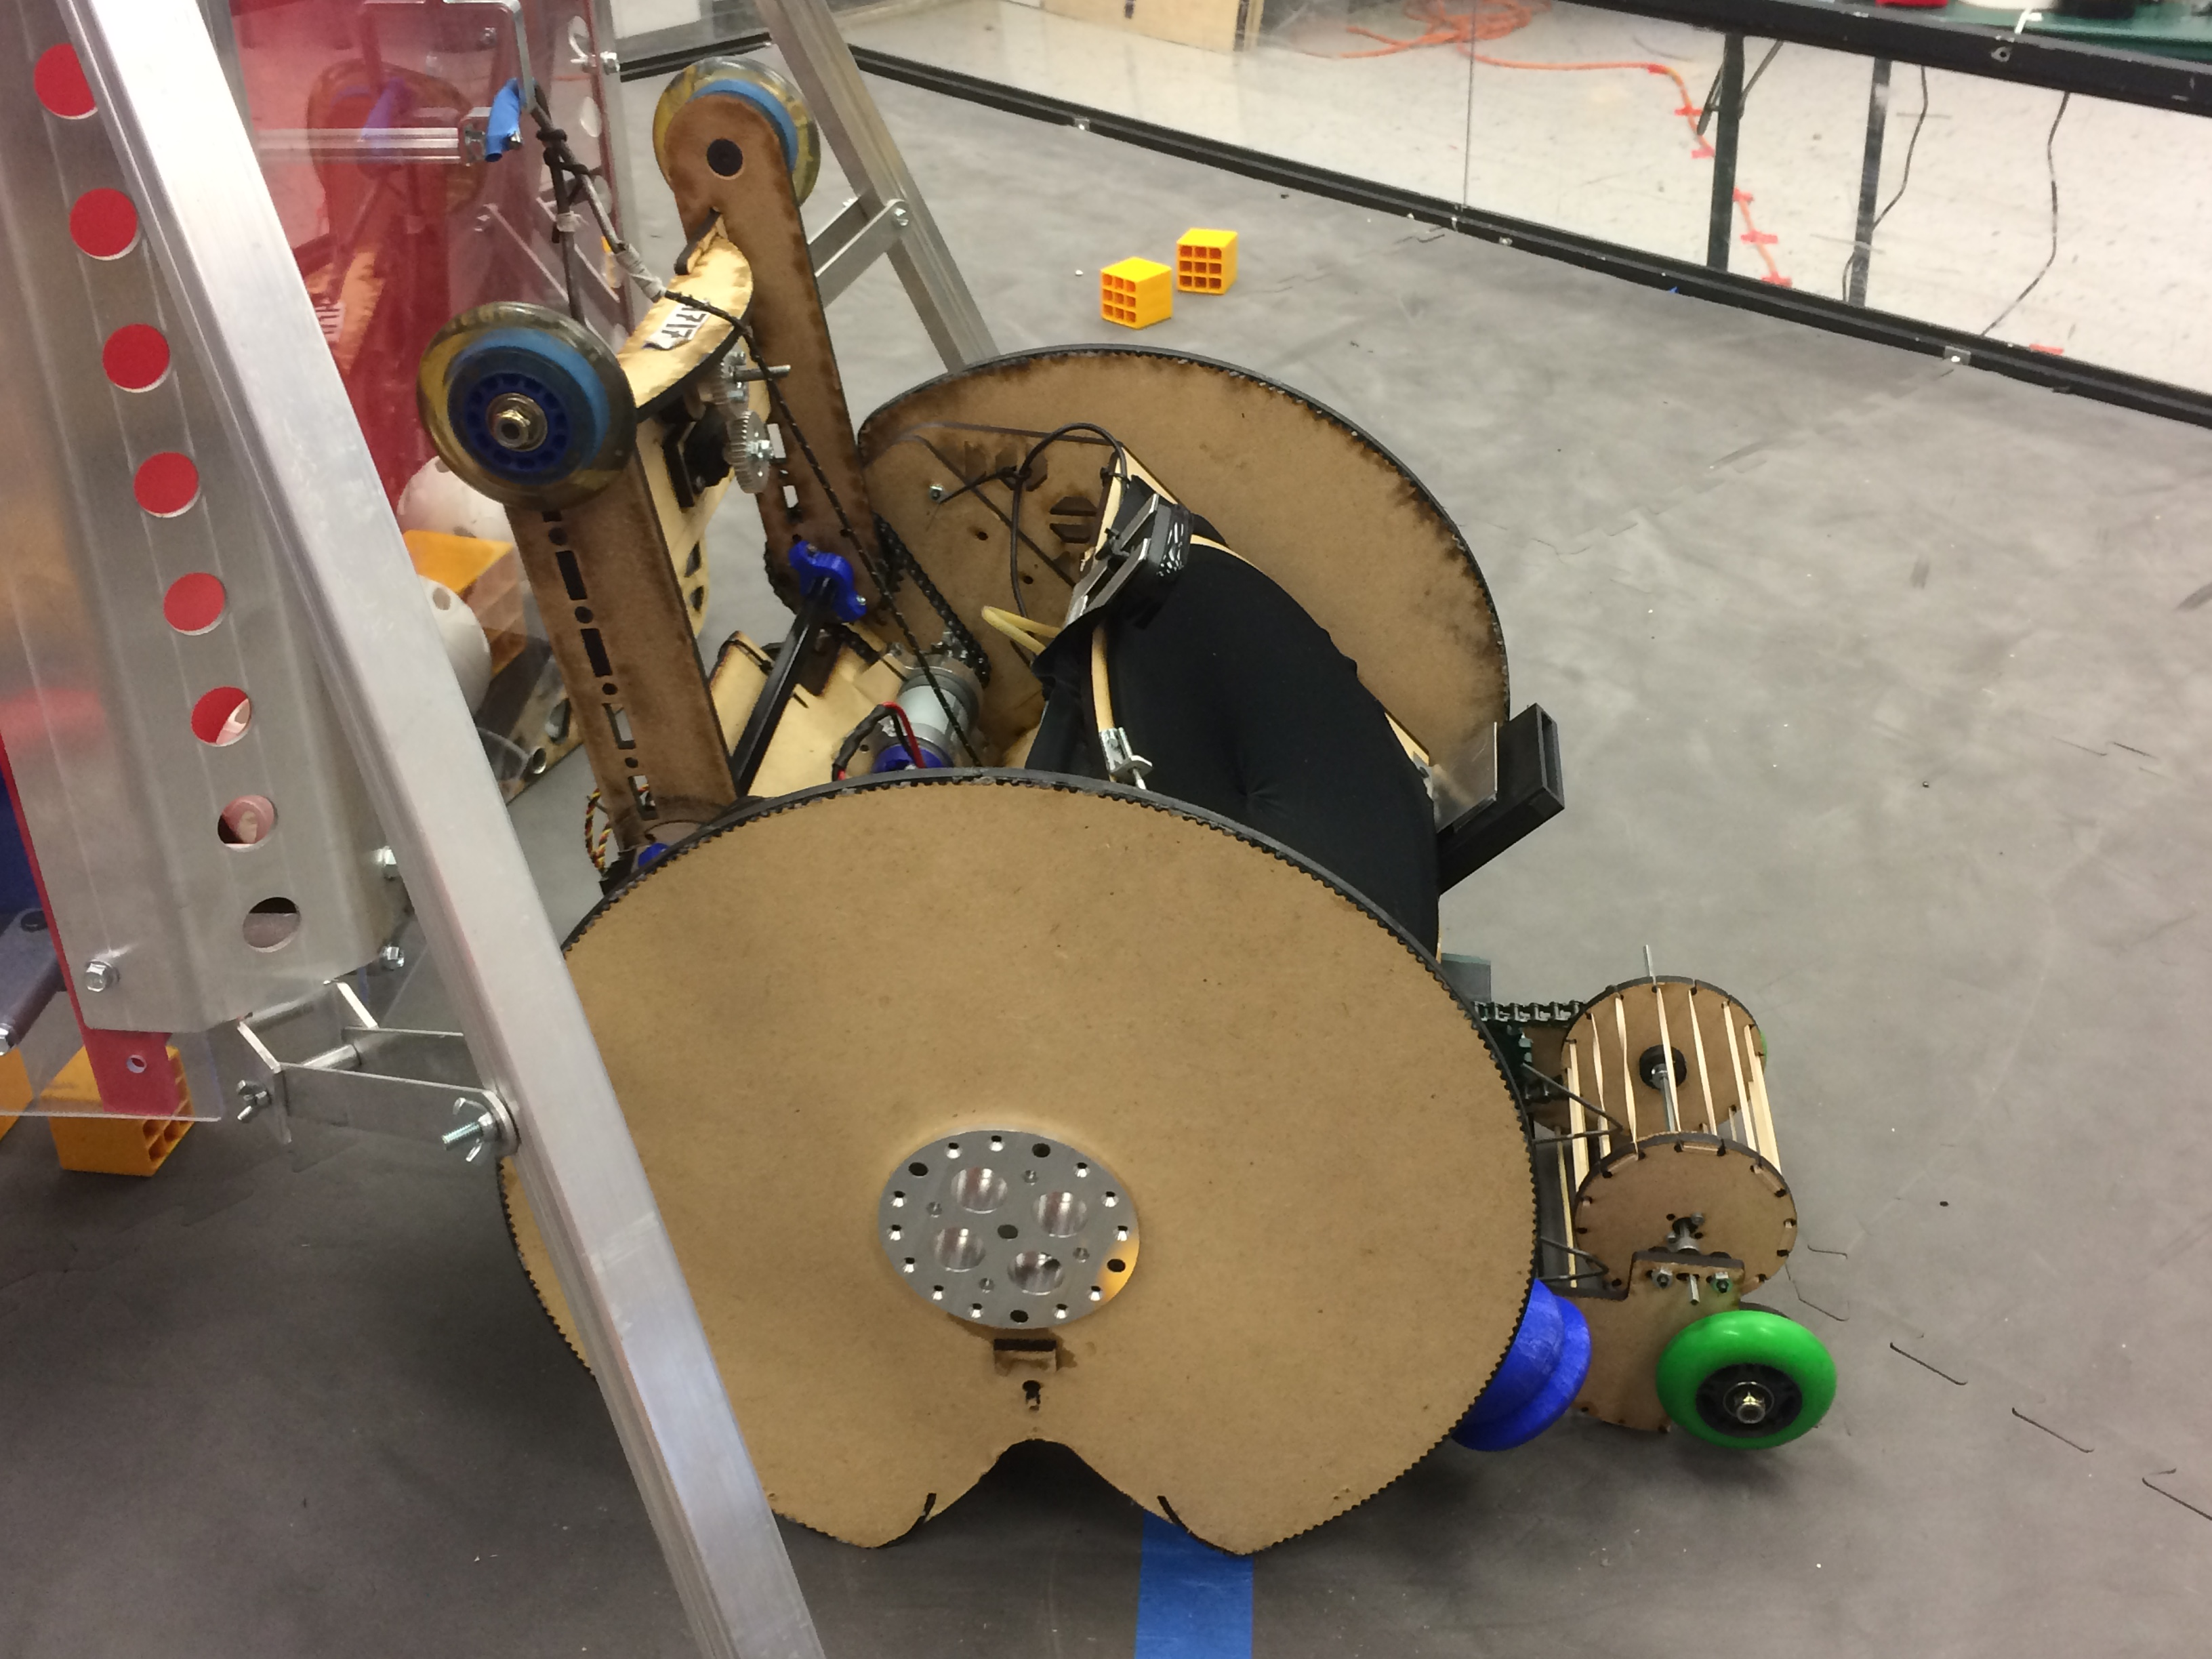
\includegraphics[width= .9\linewidth]{Design_Overview/hang_angle.JPG} %%shooting
% \end{minipage}%
%   \hfill
% \begin{minipage}{.32\textwidth}
%   \centering
%   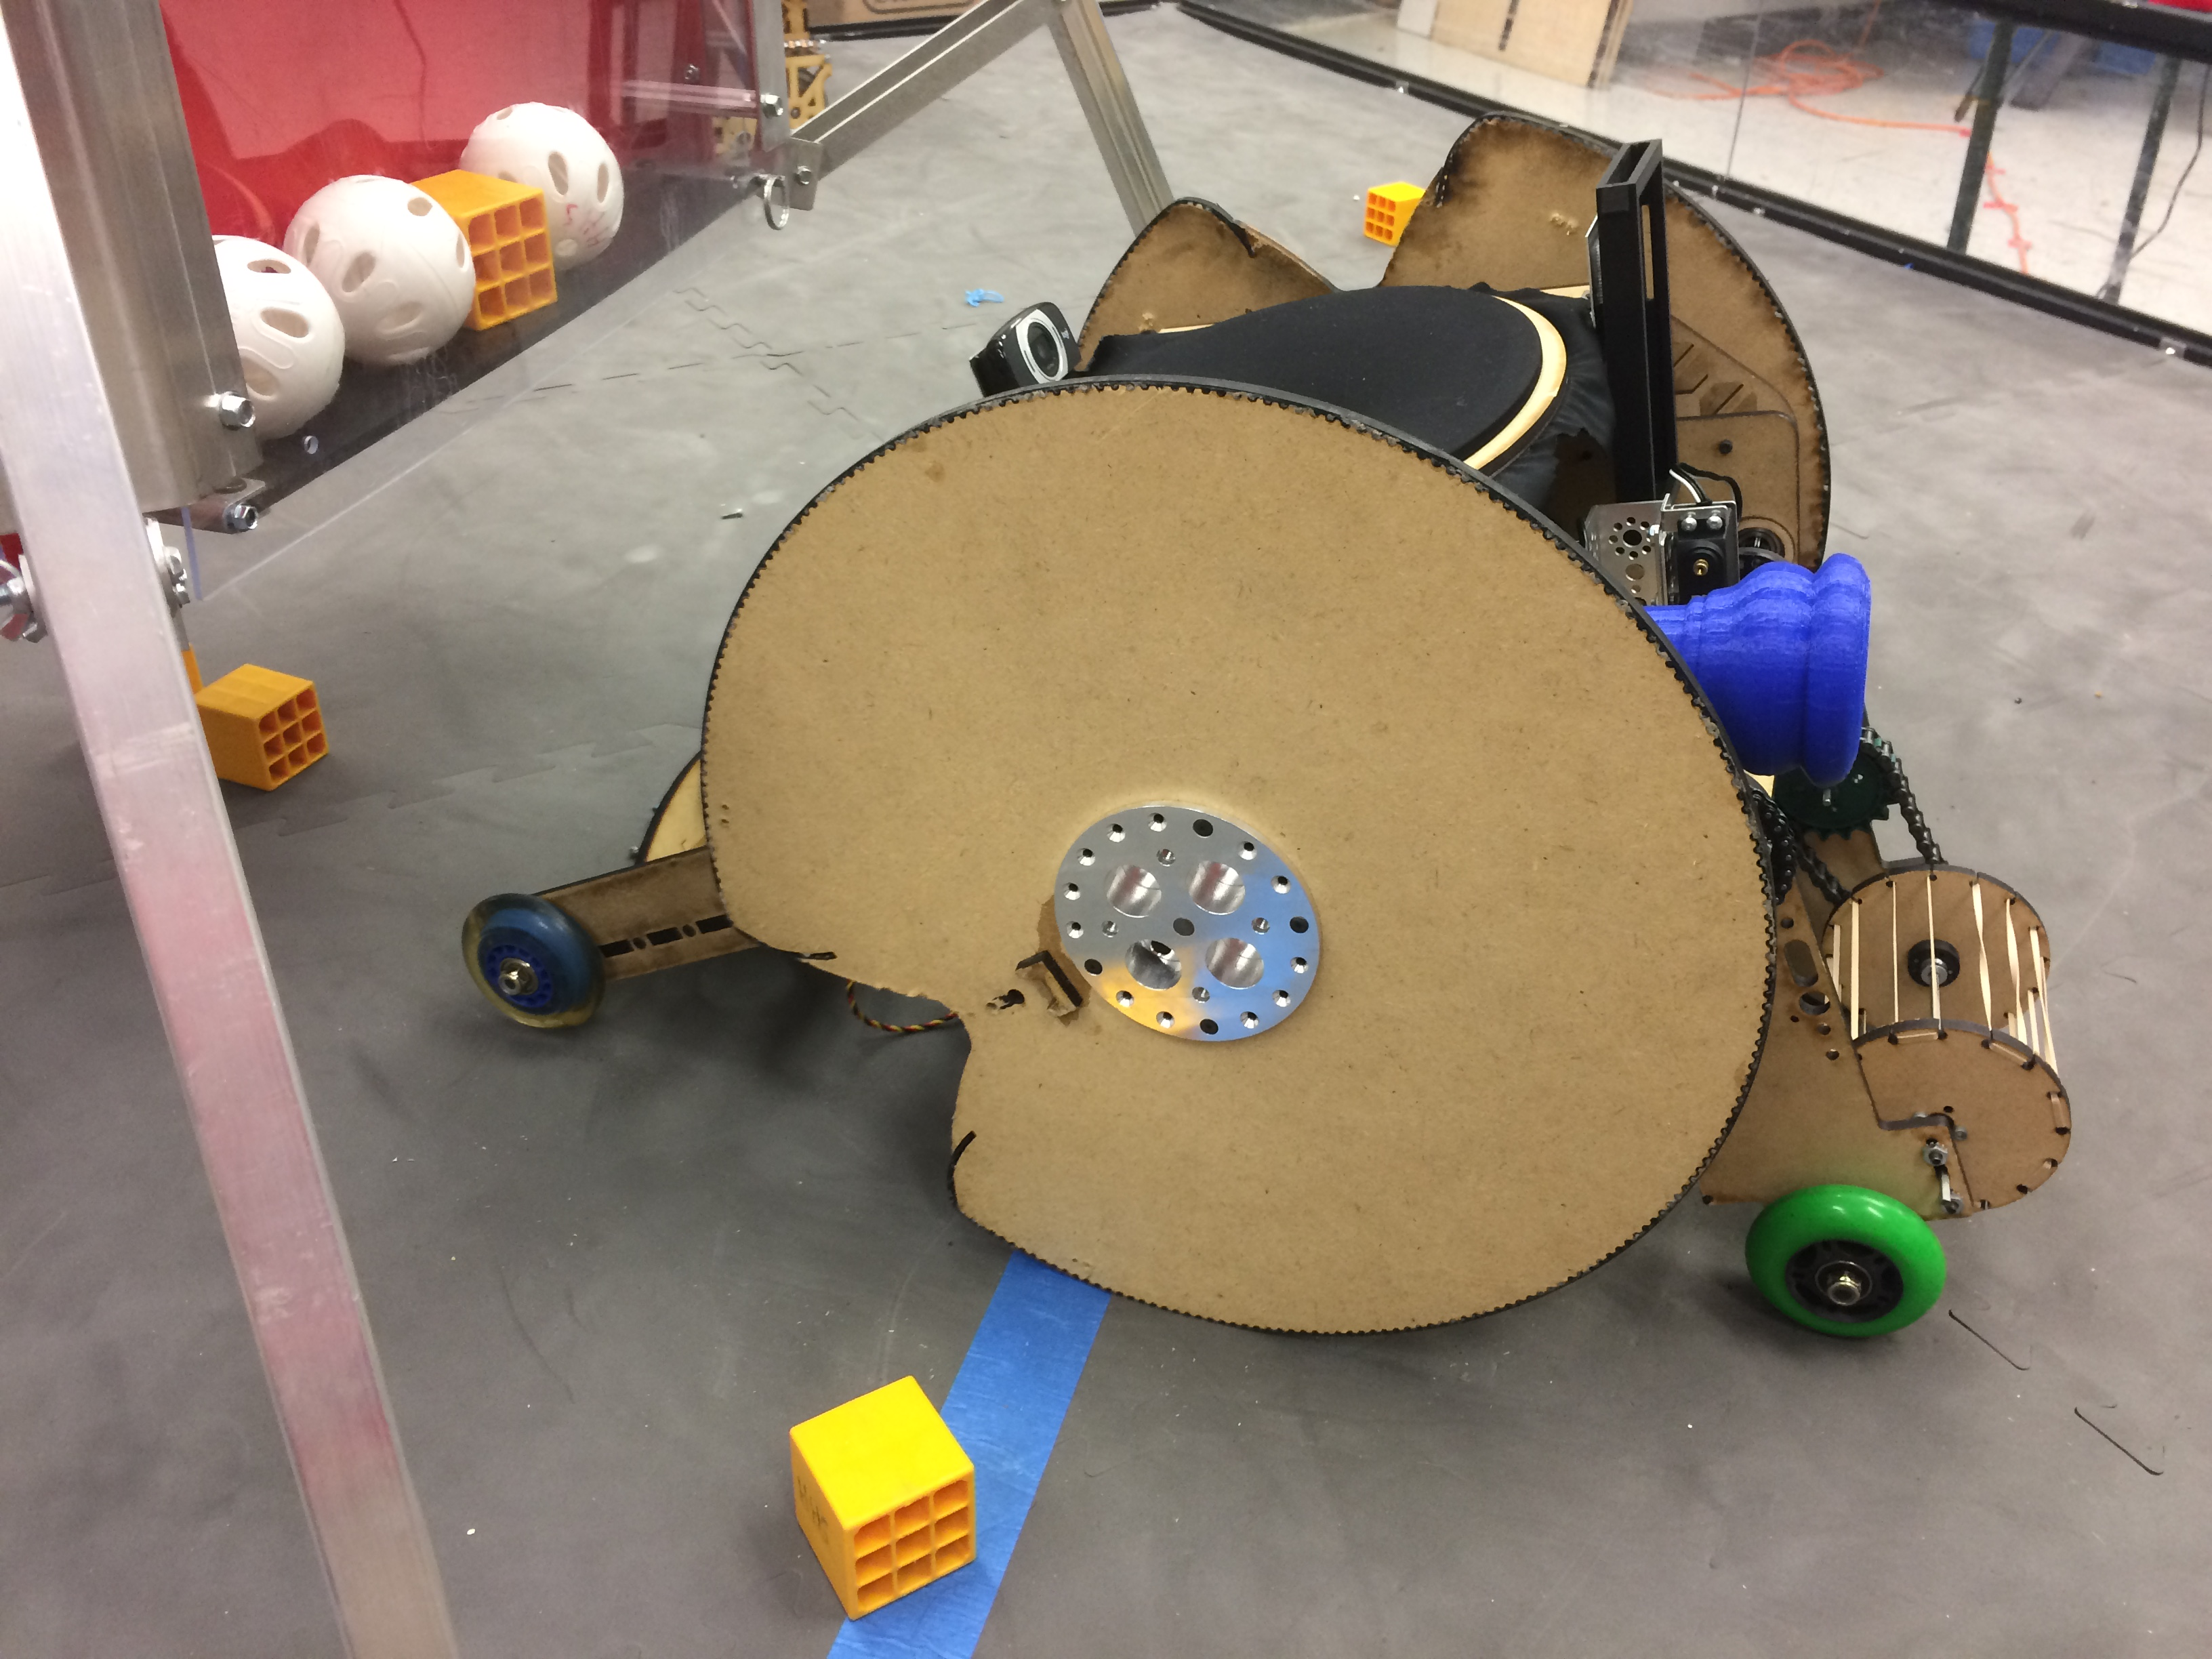
\includegraphics[width= .9\linewidth]{Design_Overview/shooter_angle.JPG} %%hang
% \end{minipage}
% \end{figure}

% \vskip 0.25in
% Chassis Stabilization and Level Driving Angles: 
% \vskip 0.05in
% \textit{
% \\The goal is to maintain ground contact of both stabilization arms in order to drive smoothly. 
% }

% \vskip 0.2in
% \begin{equation}
% \phi_{front} = \arccos(\frac{sin(\theta) + 6.7 + 6.5}{8.0} - 90 + \theta)
% \end{equation}

% \begin{equation}
% \phi_{back} = \arccos(\frac{-sin(\theta) + 6.7 + 6.5}{8.0} + 90 + \theta)
% \end{equation}

% \subsection*{Equation Analysis}
% \textit{
% \\ With the use of one of the angles, we can calculate the angle of the other arm to be stable; Refer to the January 20th entry to learn more about how these equations work, and how we created them. 
% }

% \interesting{Writing Formulas for Arm Stabilization}{control:2}

\subsection*{Mechanism Accomplishments}
\begin{itemize}
    \item alluminum material maintains strength
    \item carbon fiber sides preserve weight
    \item sleek wire management design 
  
\end{itemize} 